\chapter{Results and Discussion} \label{ch:results}

This chapter evaluates the model at three levels. First, the individual distance, azimuth, and elevation pathways are tested to determine whether the hand-designed biological abstractions produce useful coordinate estimates. This will also discuss possible solutions to predictable readout errors, which we correct with `warping'. Second, the Continuous Attractor Neural Network (CANN) readouts are compared with direct centre-of-mass readouts to determine whether the SC-like attractor improves the population code. Third, the full three-dimensional system is tested using both fixed readouts and trainable SNN fusion, including comparisons against SNN baselines that receive less structured inputs.

The emphasis is on the most informative results rather than every diagnostic experiment. The central question is whether the biologically structured pathway model provides useful intermediate representations, and whether the final trainable readout improves the model by combining these representations rather than replacing them.

\section{Evaluation Metrics}

Each model predicts distance, azimuth, and elevation. Distance errors are reported in metres or centimetres, while angular errors are reported in degrees. For full-system tests, the spherical prediction is also converted into a Cartesian point and evaluated using Euclidean position error:
\begin{equation}
    e_{\mathrm{3D}}
    =
    \left\|
        \hat{\mathbf{p}} - \mathbf{p}
    \right\|_2 ,
\end{equation}
where $\mathbf{p}$ is the true Cartesian target position and $\hat{\mathbf{p}}$ is the predicted Cartesian position.

The trainable readout experiments also report a dimensionless combined error. This is the loss-style summary used during readout comparison. It combines normalised distance error and angular sine/cosine error, so it should be interpreted as a relative comparison between readouts rather than a physical unit. Lower values indicate better overall coordinate prediction.For each sample $i$, the combined normalised error is:
\begin{equation}
    e_{\mathrm{comb},i}
    =
    \frac{1}{3}
    \left(
        \frac{|\hat{r}_i-r_i|}{r_{\max}}
        +
        \frac{|\Delta \hat{\theta}_i|}{\theta_{\max}}
        +
        \frac{|\Delta \hat{\psi}_i|}{\psi_{\max}}
    \right),
\end{equation}


and the reported value is the mean over the test set:

\begin{equation}
    E_{\mathrm{comb}}
    =
    \frac{1}{N}
    \sum_{i=1}^{N}
    e_{\mathrm{comb},i}.
\end{equation}


where: $r_i$, $\hat{r}_i$ are true and predicted distance, $\Delta \hat{\theta}_i$ is the signed angular azimuth error (wrapped, however this is less applicable for our constrained space), $\Delta \hat{\psi}_i$ is the signed elevation error, and $N$ is the number of test samples.

In the constrained final-model tests:
\begin{equation}
    r_{\max}=5\,\mathrm{m}, \quad
    \theta_{\max}=45^\circ, \quad
    \psi_{\max}=45^\circ, \quad
\end{equation}

\section{Distance Pathway}

The distance pathway was evaluated by comparing the direct feed-forward population readout against two line-attractor variants. The direct readout uses the sharpened AC distance population and decodes distance by COM. The CANN variants apply the finite line attractor before decoding: one with a diagonal input matrix and one with the reflected Gaussian input construction described in Chapter \ref{ch:modelling}.

\begin{table}[H]
    \centering
    \caption{Distance pathway readout comparison. The constrained tests use the final operating range of 0.25--5~m. The expanded test extends the same pathway to 10~m.}
    \label{tab:distance_pathway_results}
    \small
    \begin{tabular}{llrrrr}
        \toprule
        Condition & Readout & MAE & RMSE & Max error \\
        \midrule
        0.25--5~m, clean & Direct COM & 3.571~cm & 4.364~cm & 11.710~cm \\
        0.25--5~m, clean & Diagonal CANN & 3.530~cm & 4.325~cm & 11.643~cm  \\
        0.25--5~m, clean & Reflected CANN & 3.539~cm & 4.307~cm & 11.591~cm  \\
        \midrule
        Full 3D, 0.25--5~m & Direct COM & 2.831~cm & 4.167~cm & 11.500~cm  \\
        Full 3D, 0.25--5~m & Diagonal CANN & 2.761~cm & 4.007~cm & 10.755~cm  \\
        Full 3D, 0.25--5~m & Reflected CANN & 2.662~cm & 3.761~cm & 9.527~cm  \\
        \midrule
        Full 3D, 0.25--10~m & Direct COM & 34.041~cm & -- & -- \\
        Full 3D, 0.25--10~m & Diagonal CANN & 34.251~cm & -- & -- \\
        Full 3D, 0.25--10~m & Reflected CANN & 34.210~cm & -- & -- \\
        \bottomrule
    \end{tabular}
\end{table}

The distance pathway performs well in the constrained 0.25--5~m region. In the full 3D constrained test, the reflected CANN improves MAE from 2.831~cm to 2.662~cm and reduces the maximum error from 11.500~cm to 9.527~cm. This is a small but consistent improvement. It supports the interpretation of the attractor as a stabilising readout rather than a replacement for the pathway itself: most of the distance information is already present in the AC population before the CANN.

The expanded 10~m test shows a different failure mode. The error increases to approximately 34~cm for all readouts, and the CANN does not correct it. This is important because it shows that the attractor cannot recover information that is not encoded reliably by the upstream pathway. The distance model was tuned for short-to-mid-range echolocation, and extending the range without retuning the cochlear thresholding, delay candidates, and suppression assumptions causes upstream degradation before the SC-like readout is reached.

The pathways were visualised to show the spiking behaviour along the pathway and readout responses:

\begin{figure}[H]
    \centering
    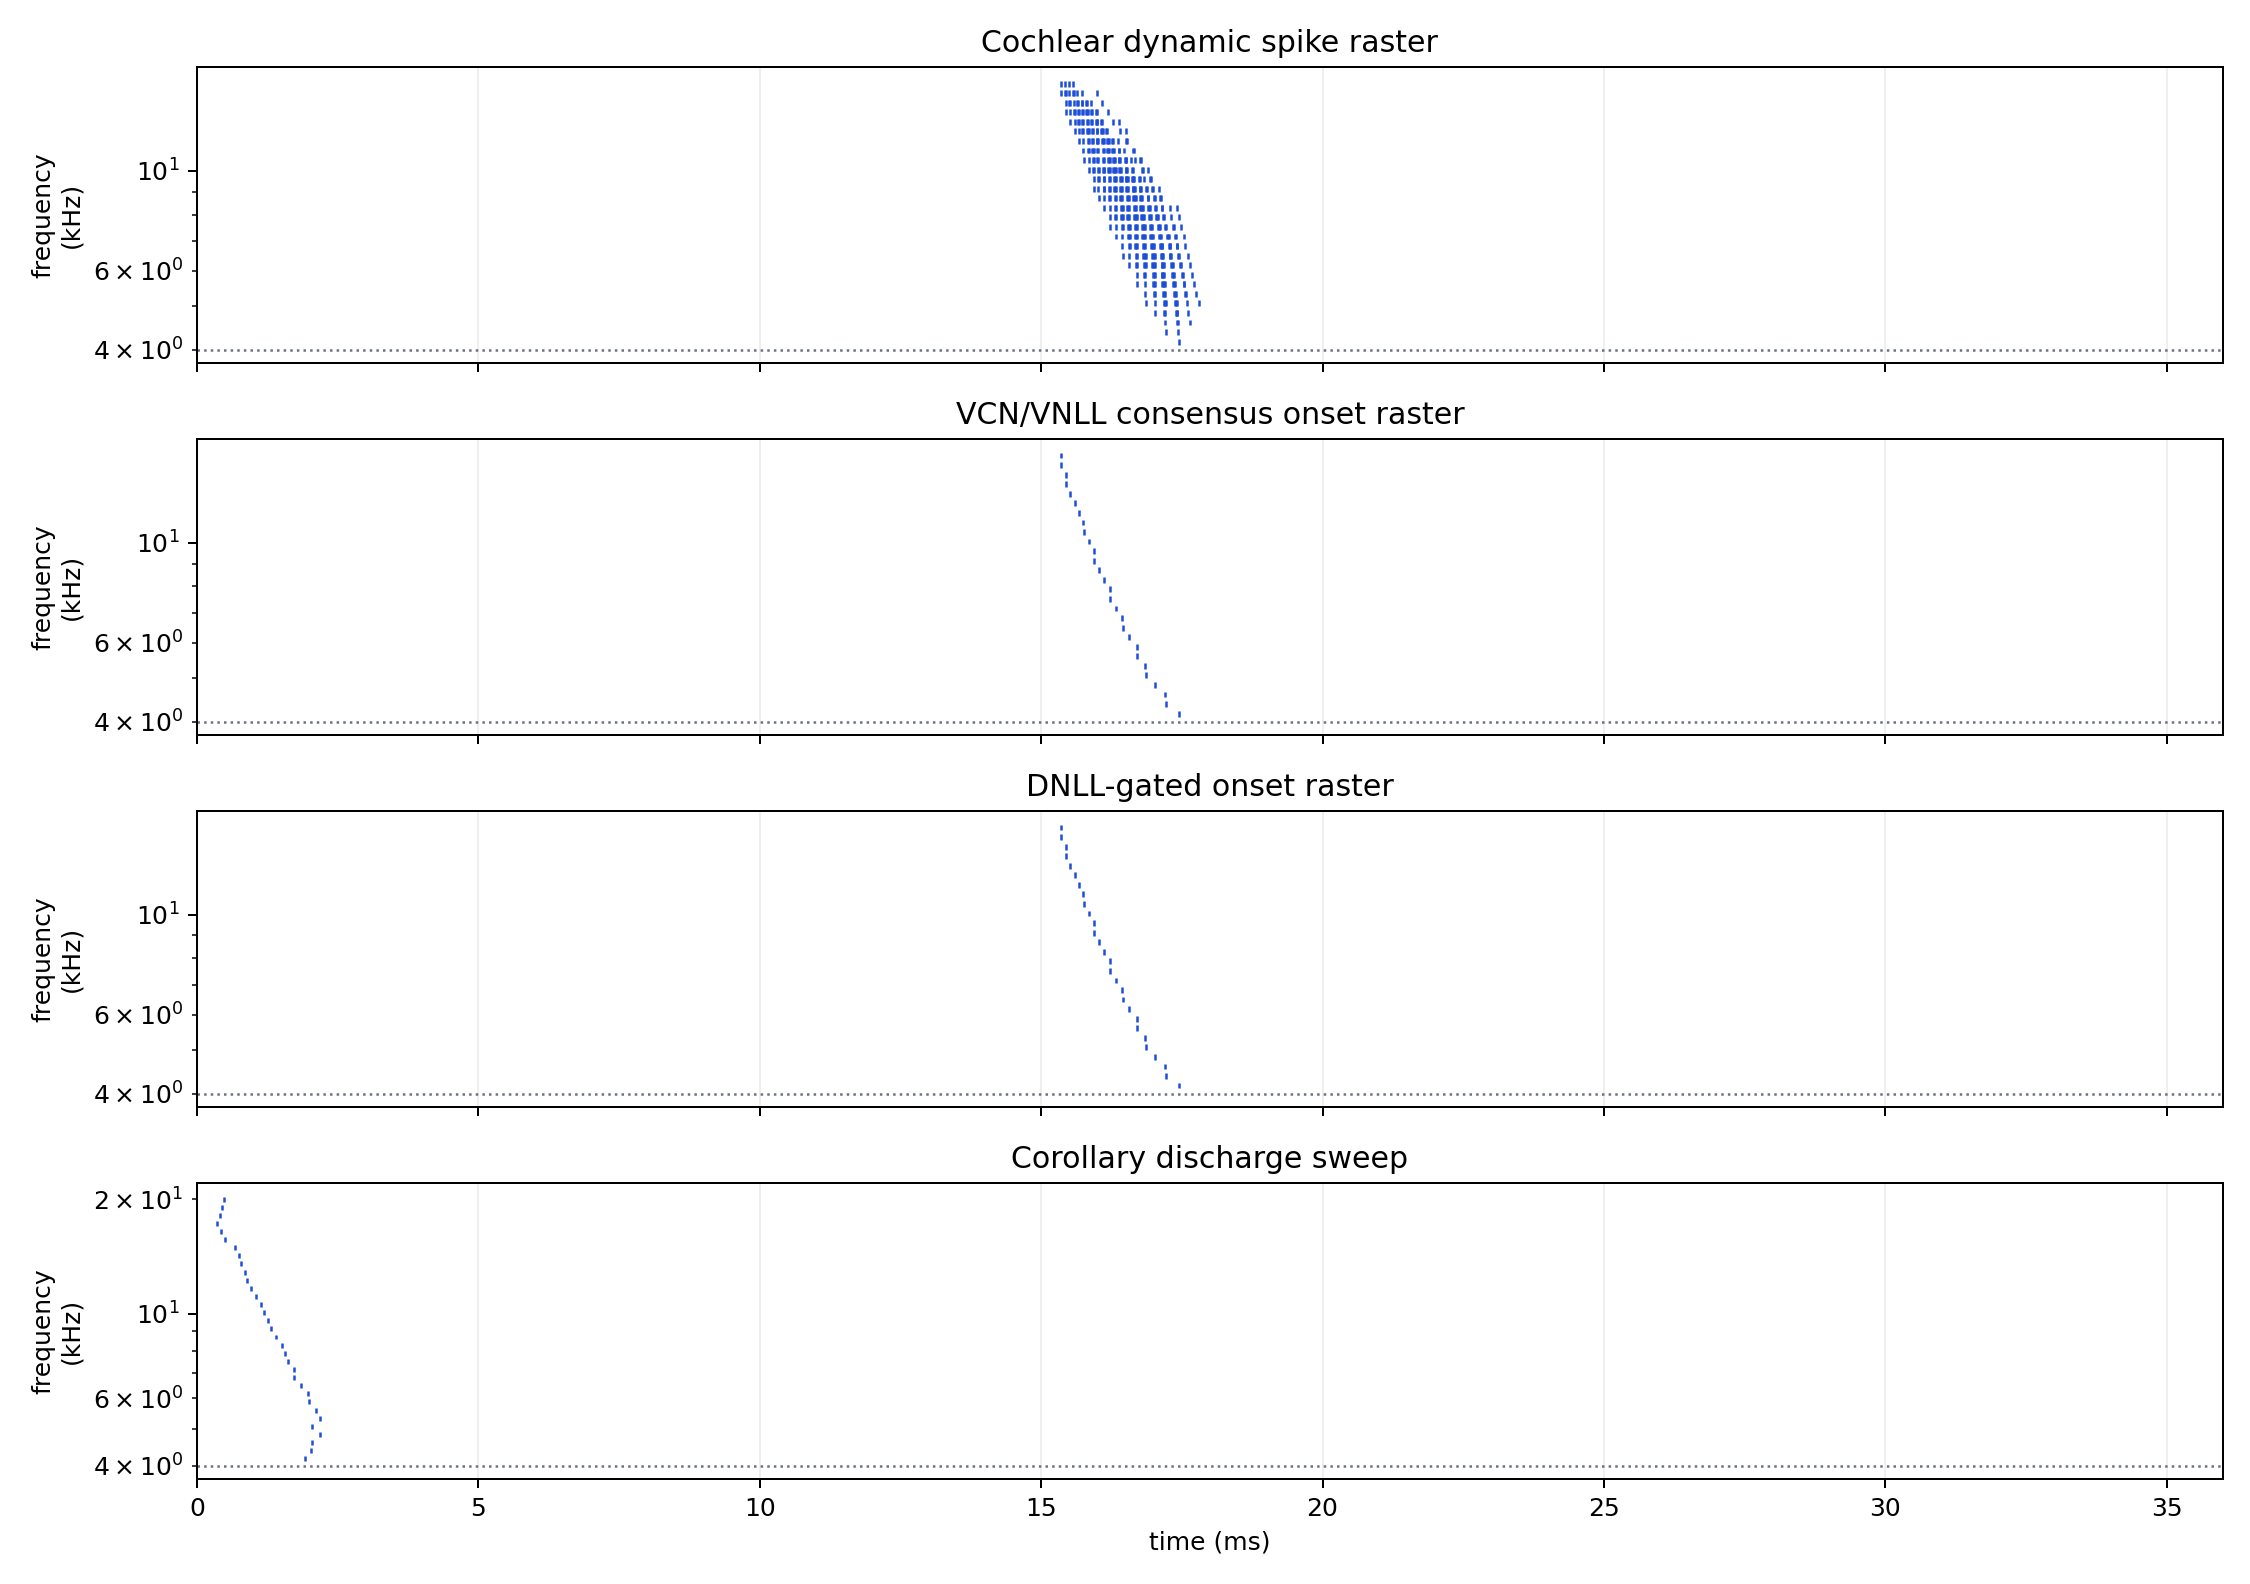
\includegraphics[width=1\textwidth]{4_Results/distance/distance_spikes.png}
    \caption{Spiking signals of cochlear spike raster, VCN/VNLL, DNLL, and corollary discharge }
    \label{fig:distance_spikes}
\end{figure}

\begin{figure}[H]
    \centering
    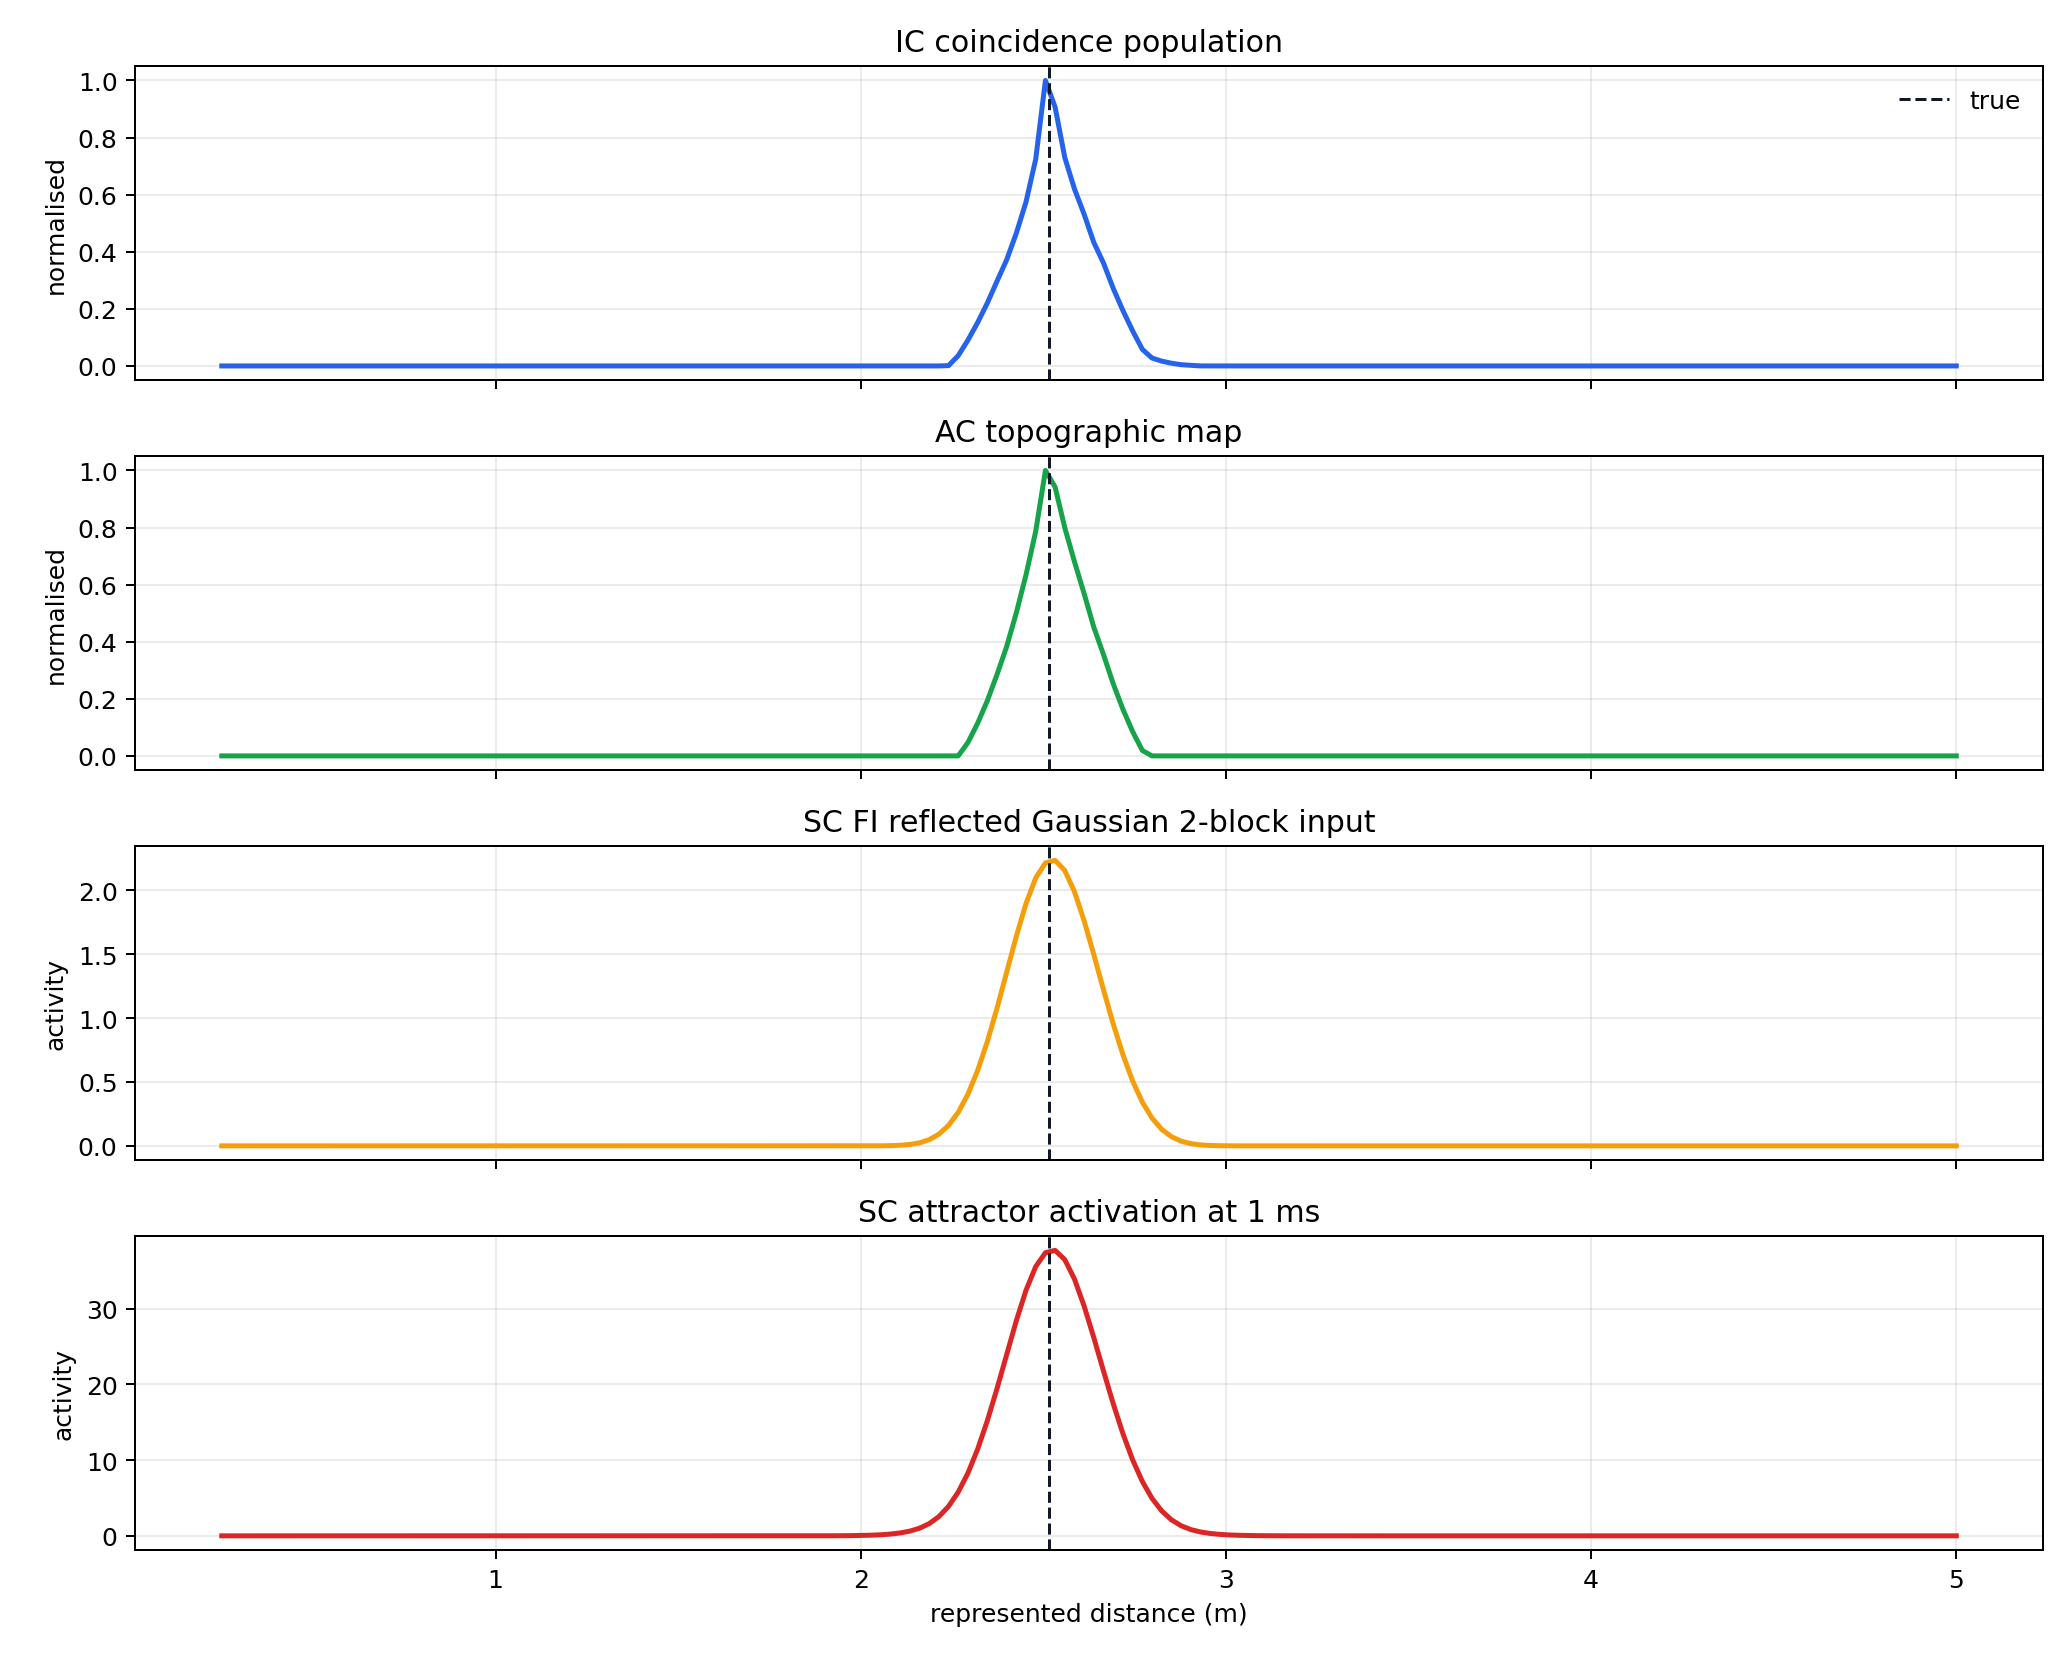
\includegraphics[width=0.7\textwidth]{4_Results/distance/distance_responses.png}
    \caption{Distance responses of IC, AC, and SC}
    \label{fig:distance_responses}
\end{figure}

\begin{figure}[H]
    \centering
    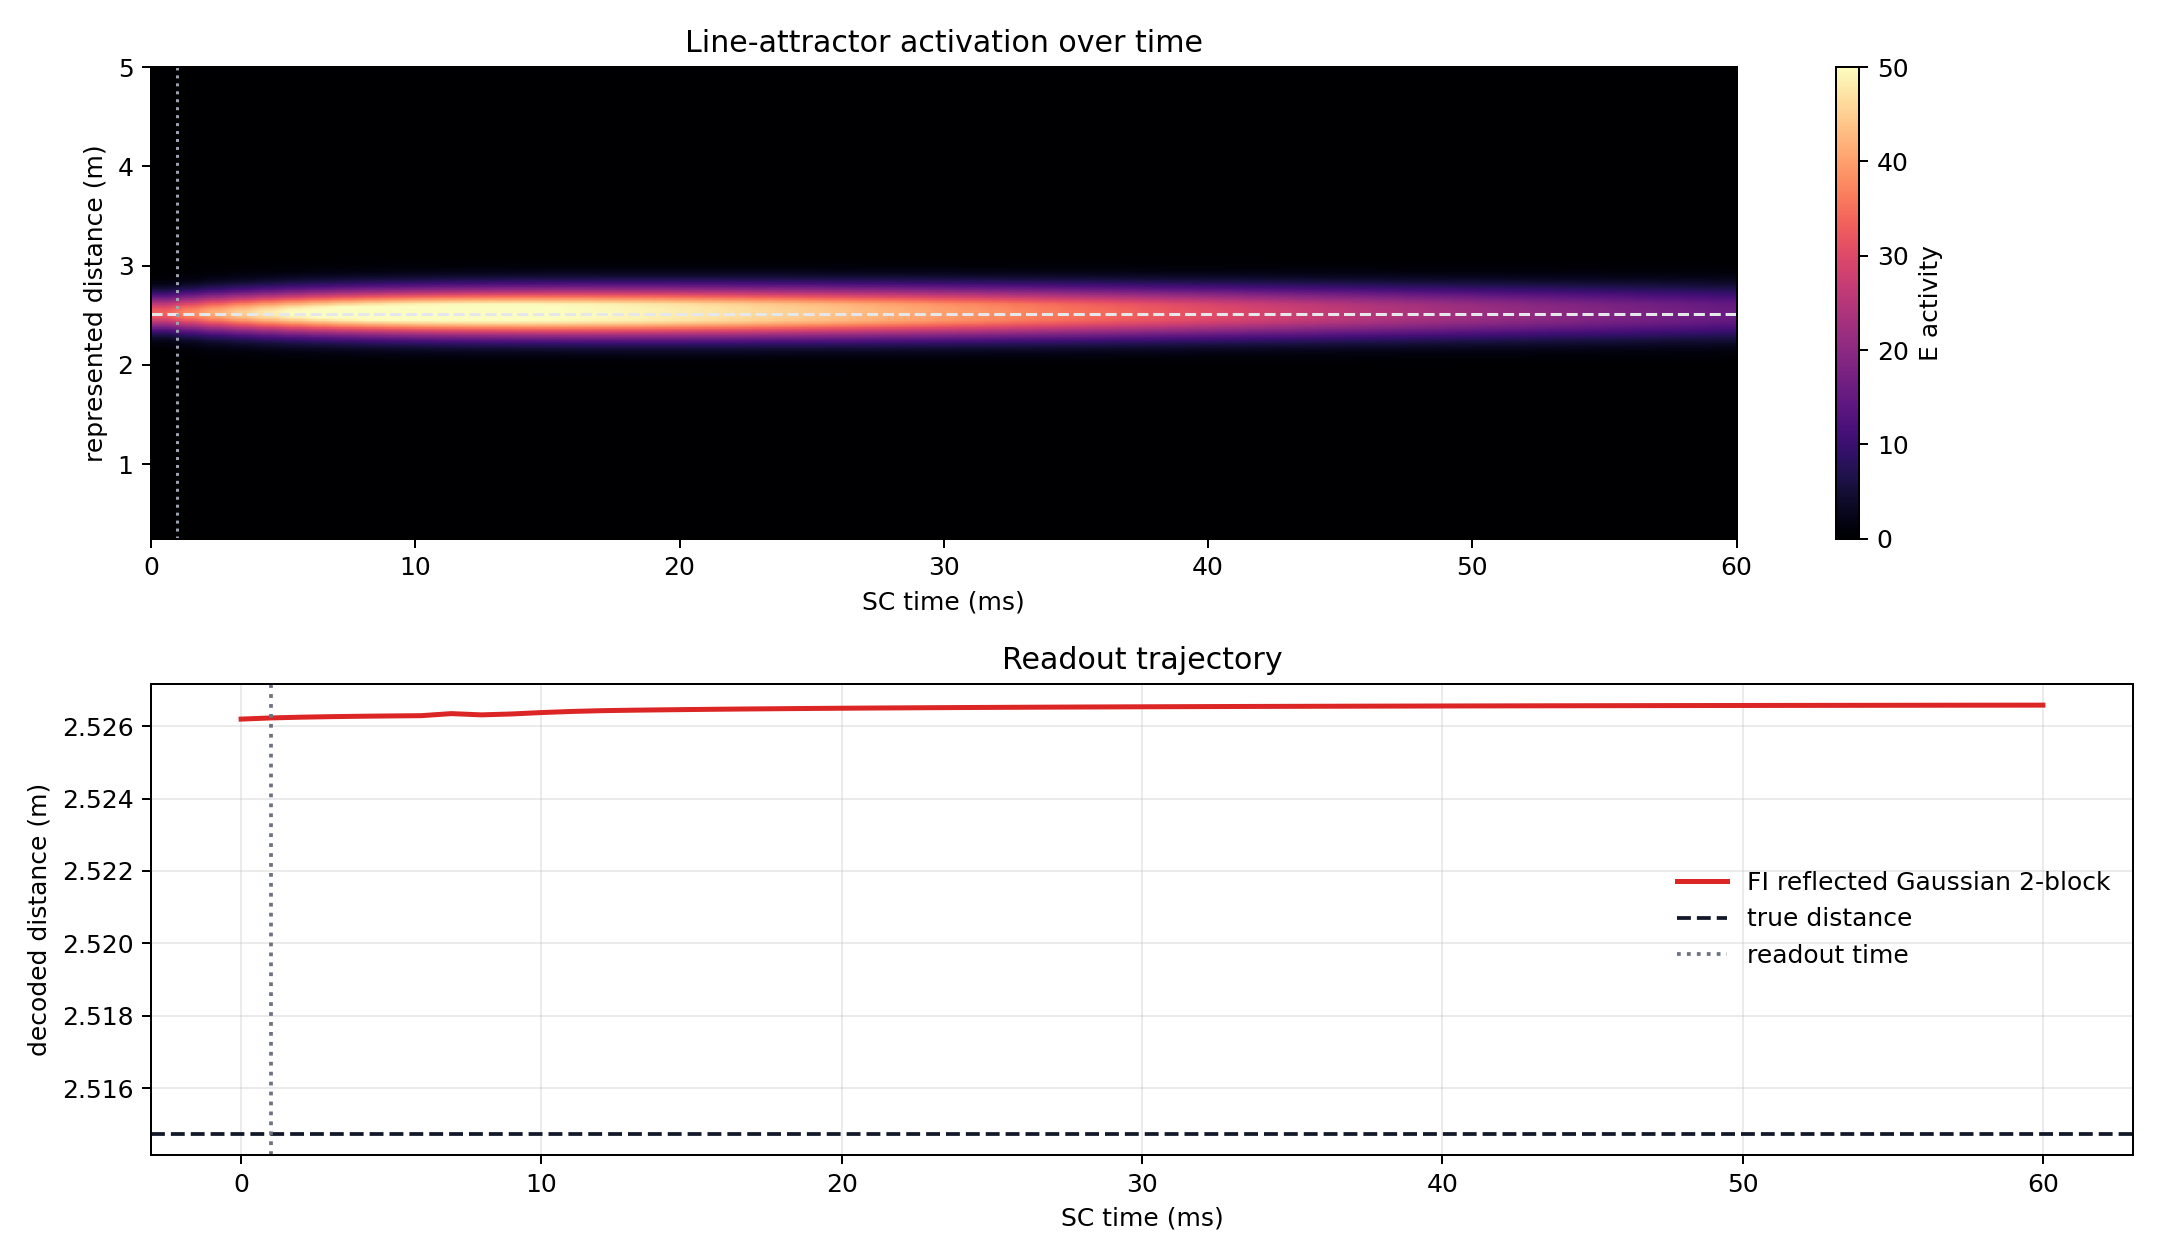
\includegraphics[width=0.7\textwidth]{4_Results/distance/distance_CANN.png}
    \caption{Response of the CANN over time}
    \label{fig:distance_CANN}
\end{figure}
\begin{figure}[H]
    \centering
    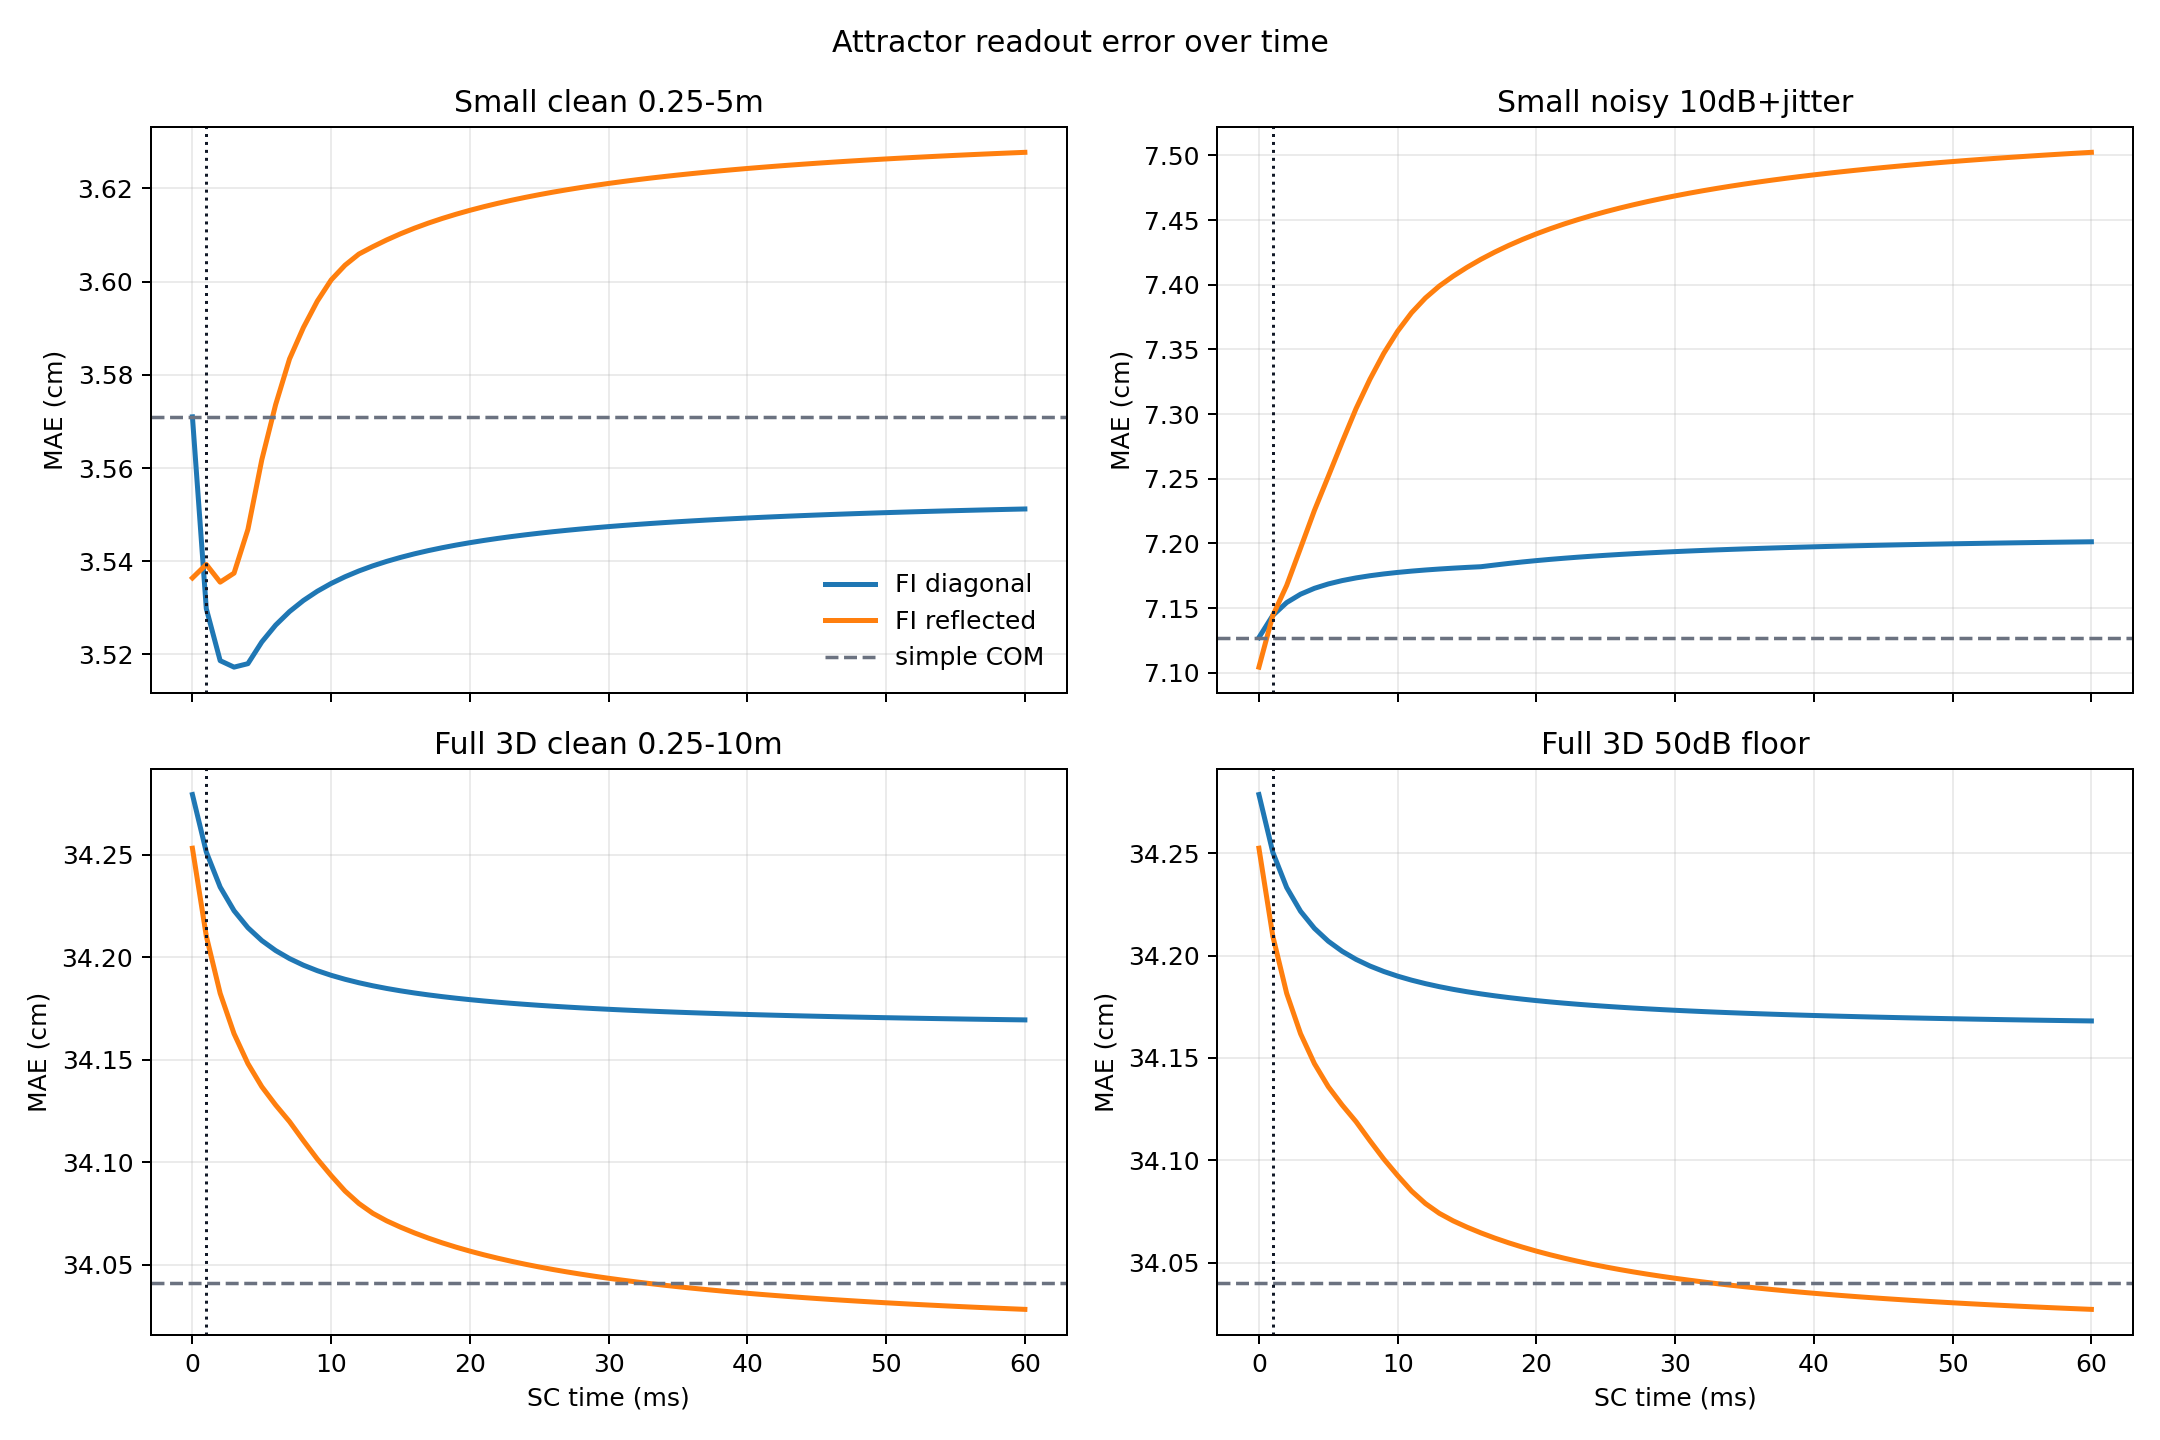
\includegraphics[width=0.7\textwidth]{4_Results/distance/distance_readout.png}
    \caption{Readouts over time of CANN models with diagonal and Gaussian inputs}
    \label{fig:distance_readouts}
\end{figure}

\section{Azimuth Pathway}

The azimuth pathway was tested using both ILD and ITD populations. The ILD branch uses opponent left/right level comparison and can be improved by an inverse-sigmoid calibration because the physical level cue saturates near the edges of the angular range. The ITD branch uses Jeffress-style onset coincidence between the two ears. In the final hand-designed model, the ITD+CANN branch is used as the main azimuth readout because it is more robust than the ILD-only readout in the constrained full-3D setting. However, both raw ITD and raw ILD populations are retained for the trainable fusion network.

\begin{table}[H]
    \centering
    \caption{Azimuth pathway comparison. Values are mean absolute azimuth error. The full-3D tests use the constrained 0.25--5~m, $\pm45^\circ$ operating region.}
    \label{tab:azimuth_pathway_results}
    \small
    \begin{tabular}{llrr}
        \toprule
        Pathway & Condition & Direct readout & CANN readout \\
        \midrule
        ILD with inverse-sigmoid calibration & Isolated $\pm45^\circ$ & 0.982$^\circ$ & 1.019$^\circ$ \\
        ILD with inverse-sigmoid calibration & Full 3D, clean & 6.175$^\circ$ & 6.127$^\circ$ \\
        ILD with inverse-sigmoid calibration & Full 3D, 50~dB noise & 6.119$^\circ$ & 6.071$^\circ$ \\
        \midrule
        ITD coincidence & Isolated $\pm45^\circ$ & 1.891$^\circ$ & 2.090$^\circ$ \\
        ITD coincidence & Full 3D, clean & 3.351$^\circ$ & 3.732$^\circ$ \\
        ITD coincidence & Full 3D, 50~dB noise & 3.349$^\circ$ & 3.718$^\circ$ \\
        \bottomrule
    \end{tabular}
\end{table}

The ILD branch gives very accurate isolated results after calibration, but its error increases in the full 3D case. This is expected because ILD is not a pure azimuth cue in the simulated full system. Distance changes overall echo amplitude, and elevation changes spectral content through the comb filter. Both effects can distort the level balance used by the LSO/MNTB abstraction.

The ITD branch is less accurate than calibrated ILD in the isolated one-dimensional test, but it is better in the constrained full-3D test. This is because onset timing is less directly affected by the elevation spectral notch and by moderate amplitude changes. The CANN does not always improve the ITD scalar readout; in these tests it slightly worsens the ITD MAE. This is not a contradiction of the attractor idea. It indicates that, for azimuth, the raw ITD population is already sharp enough and the attractor smoothing can introduce a small bias. For this reason, the final trainable readout receives both the raw populations and the CANN readout, allowing it to learn when the attractor output is useful and when the raw population should dominate.

\begin{figure}[H]
    \centering
    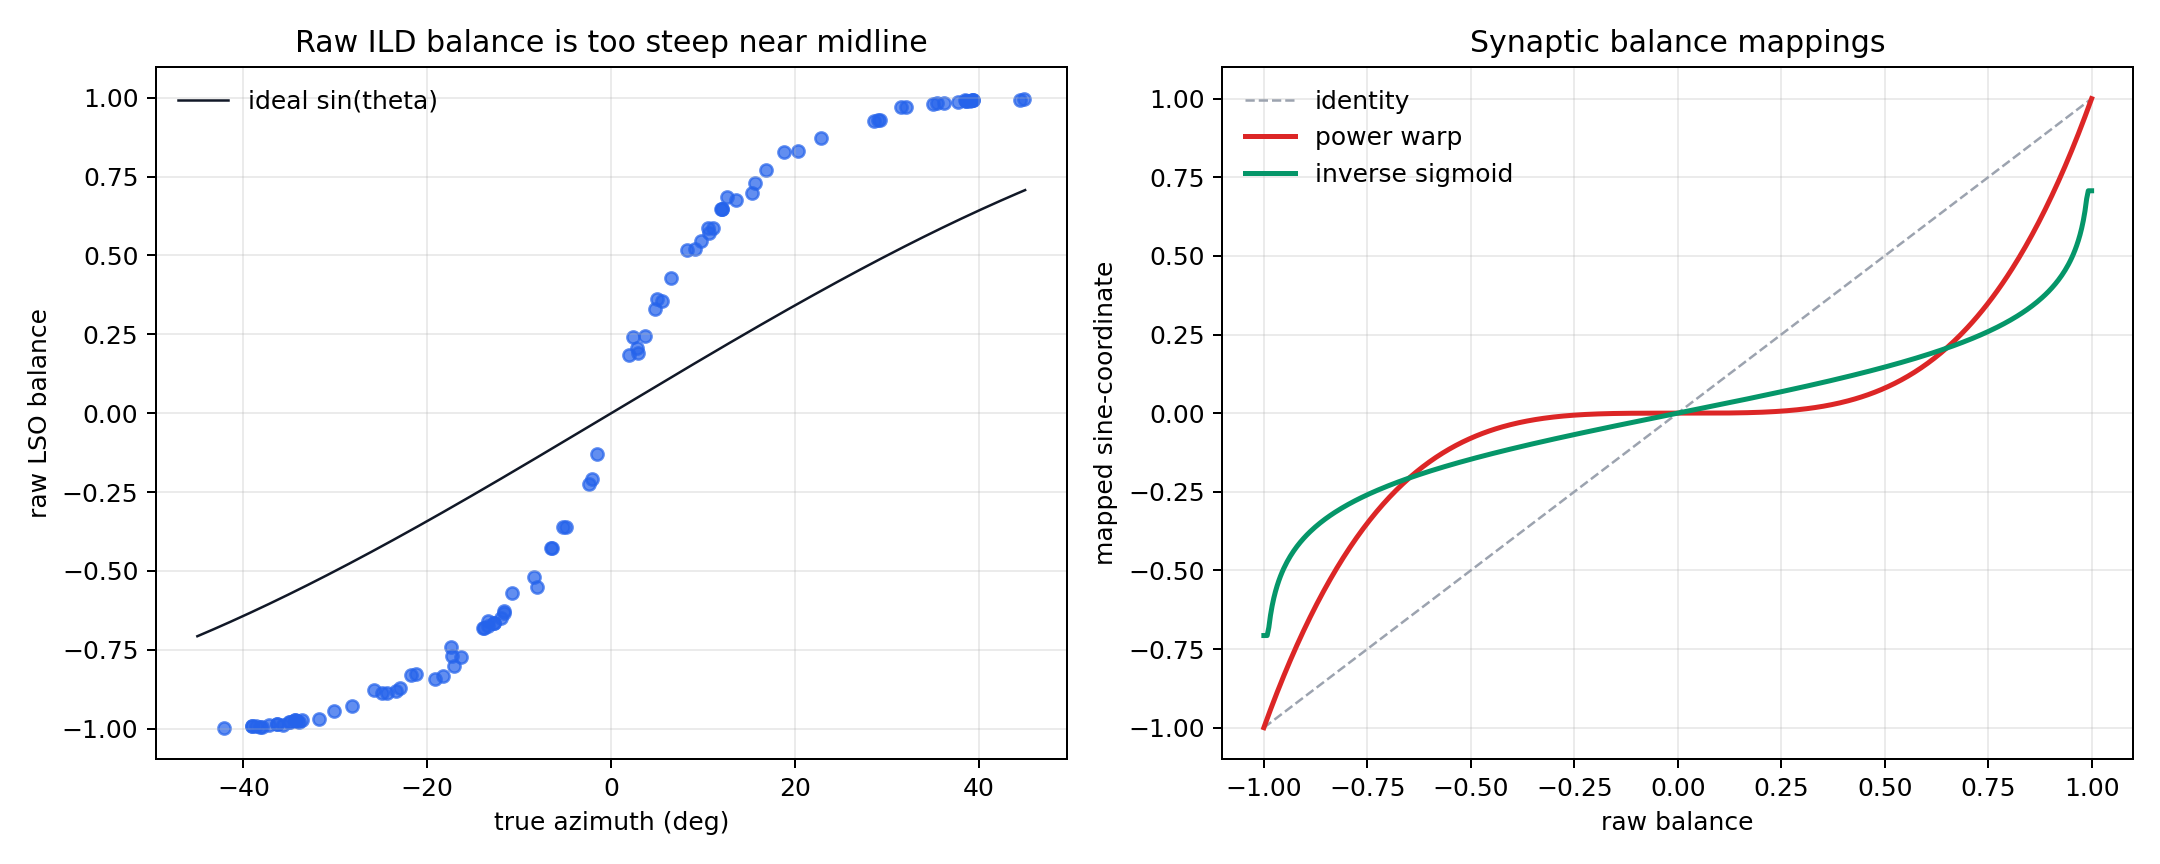
\includegraphics[width=1\textwidth]{4_Results/azimuth/ILD_warp.png}
    \caption{ILD-based azimuth scatter plot showing a systematic, predictable error, and proposed warping functions}
    \label{fig:ILD_warp}
\end{figure}

\begin{figure}[H]
    \centering
    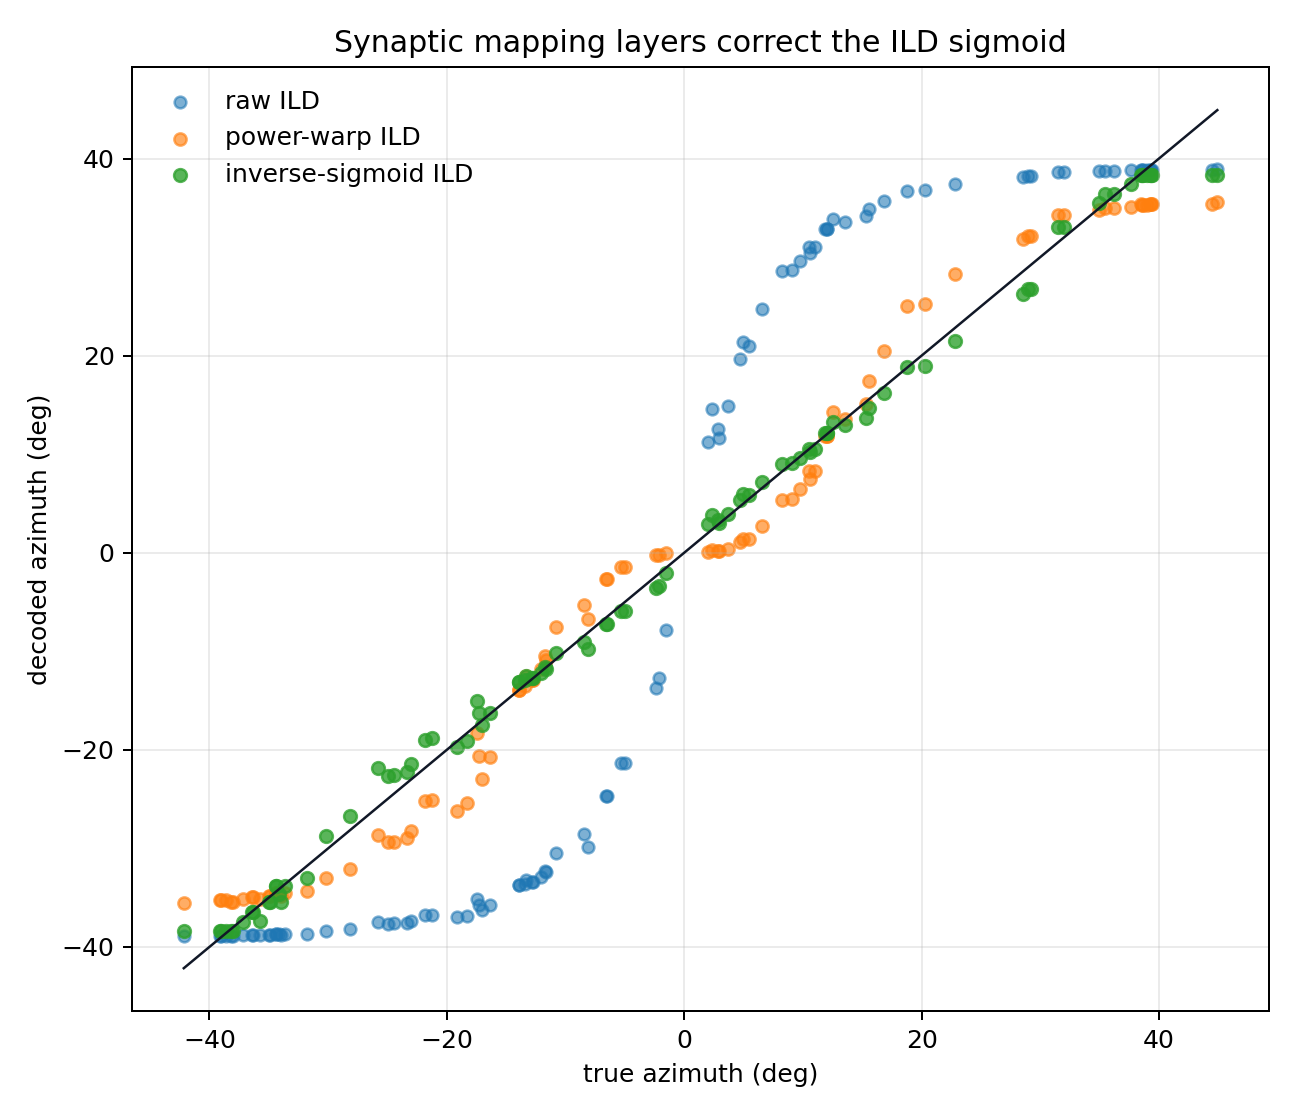
\includegraphics[width=0.6\textwidth]{4_Results/azimuth/warp_scatter.png}
    \caption{Scatter plot showing effect of warping}
    \label{fig:warp_scatter}
\end{figure}


\begin{figure}[H]
    \centering
    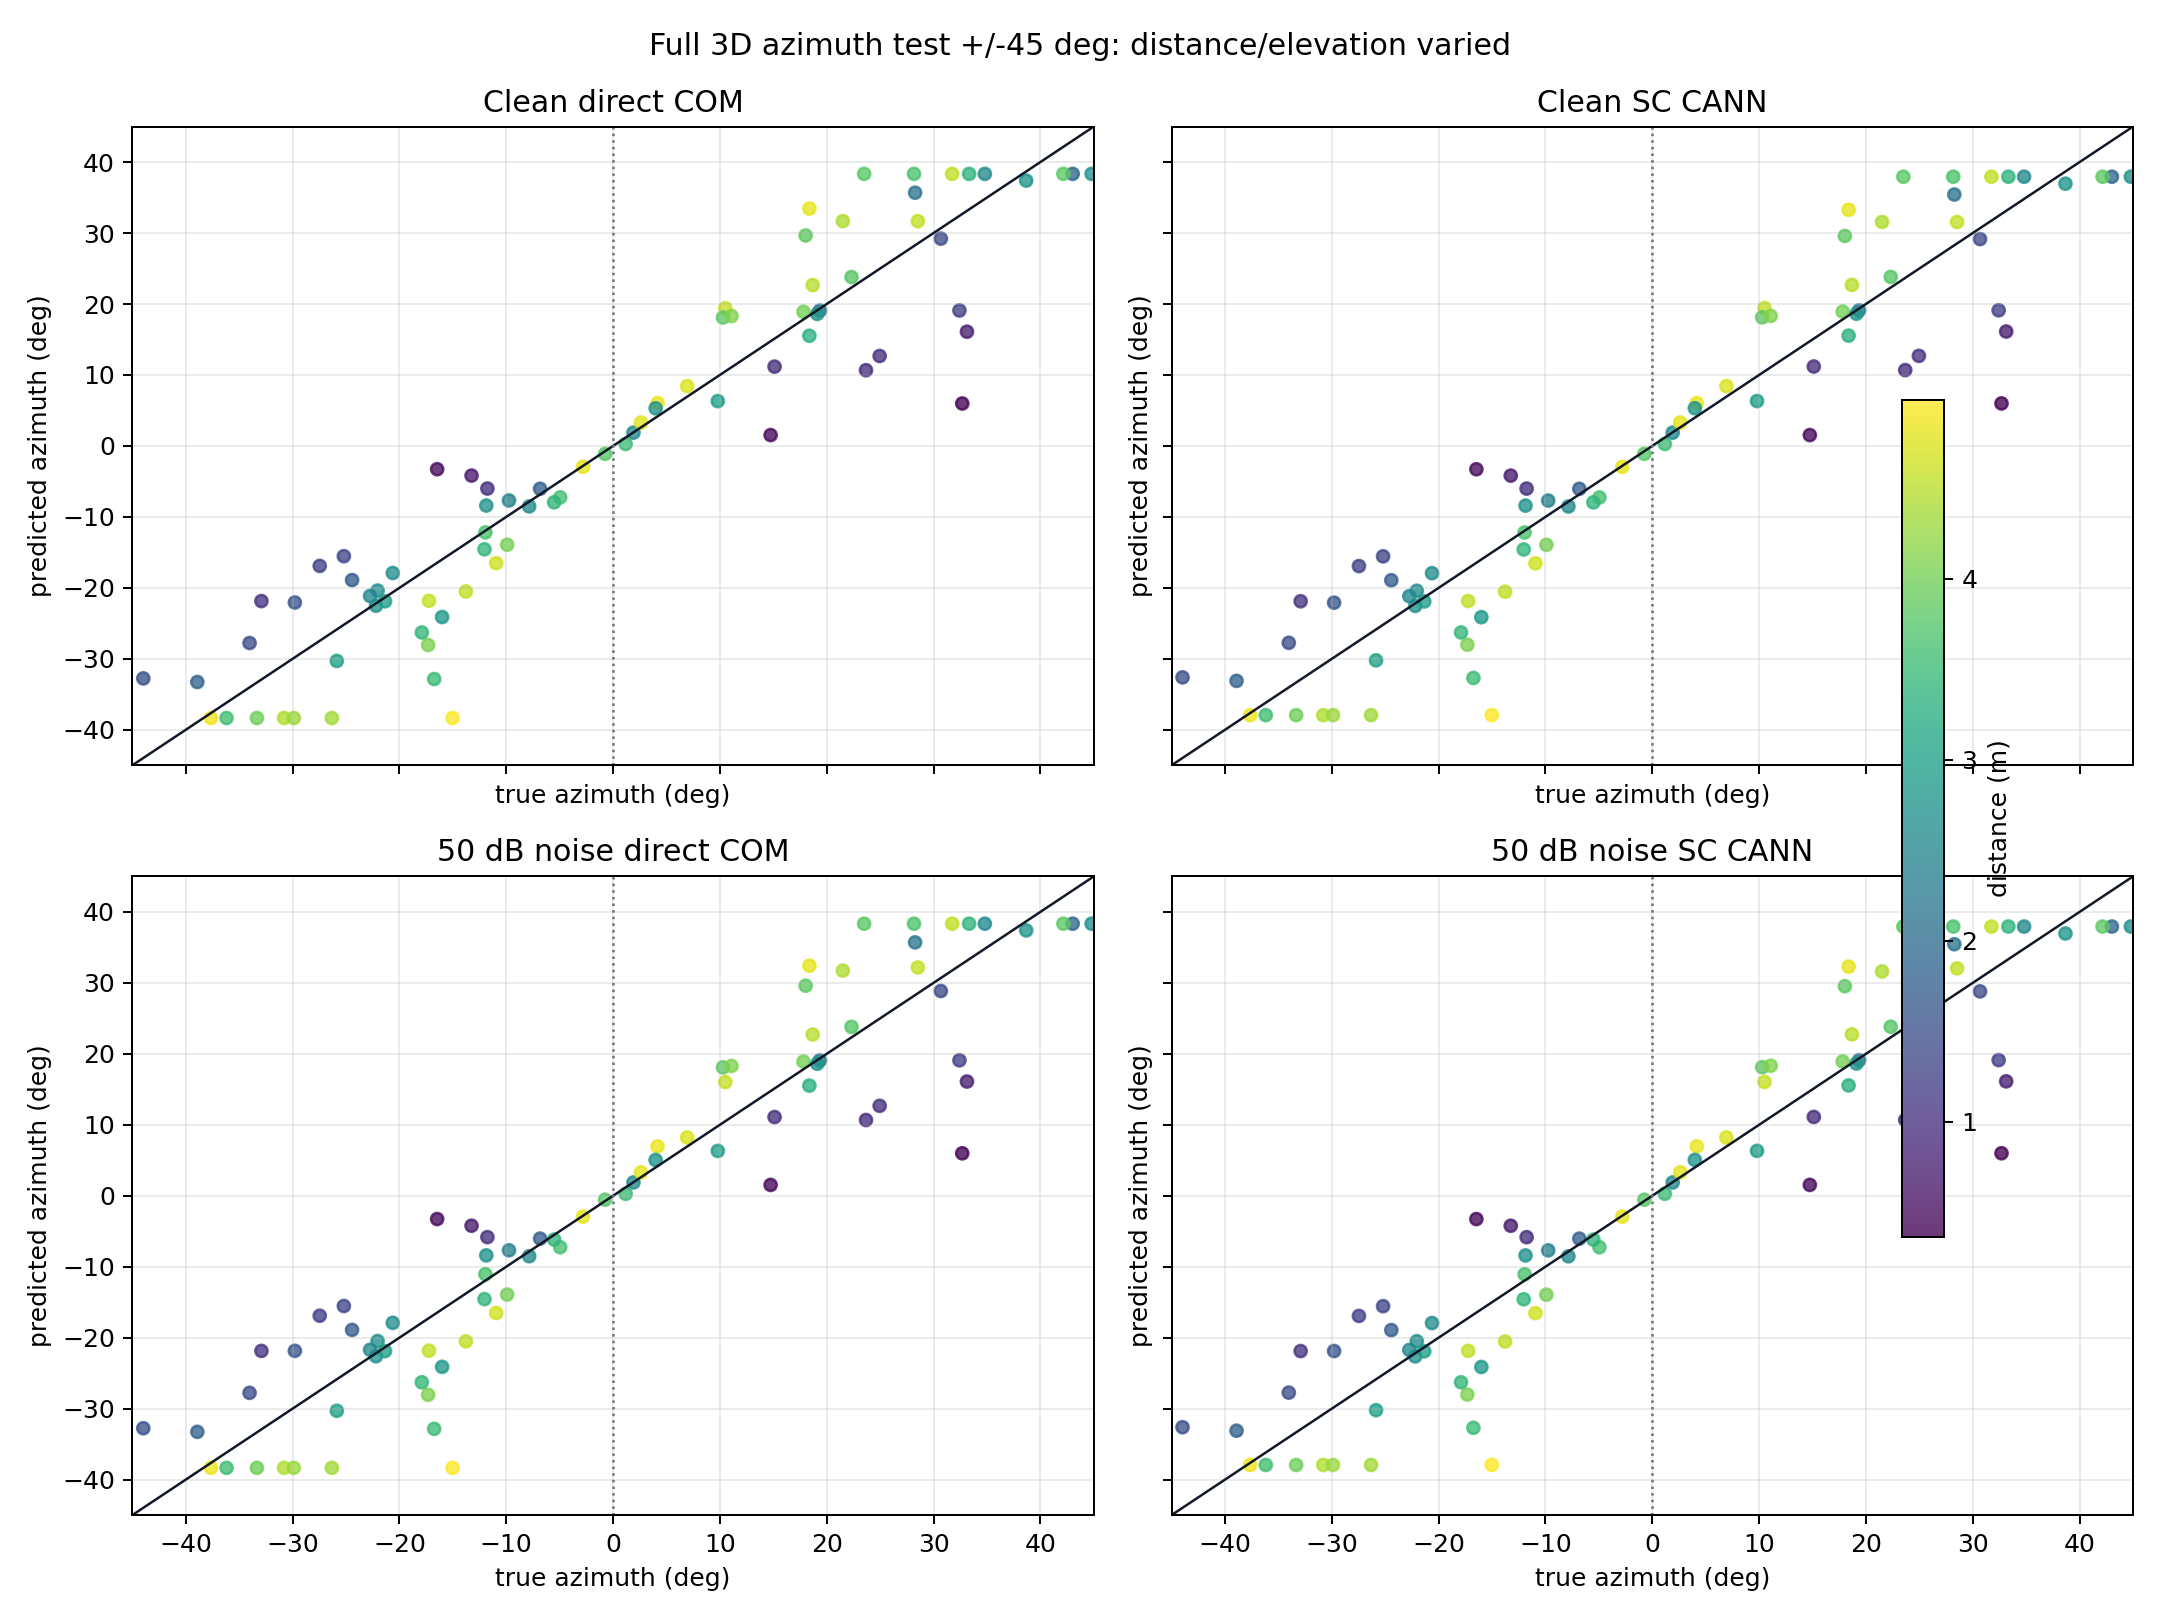
\includegraphics[width=1\textwidth]{4_Results/azimuth/ILD_scatter.png}
    \caption{Scatters showing results of ILD based azimuth estimation for constrained 3D environment, with direct and CANN readouts, in clean and noisy environments}
    \label{fig:ILD_warp}
\end{figure}

\begin{figure}[H]
    \centering
    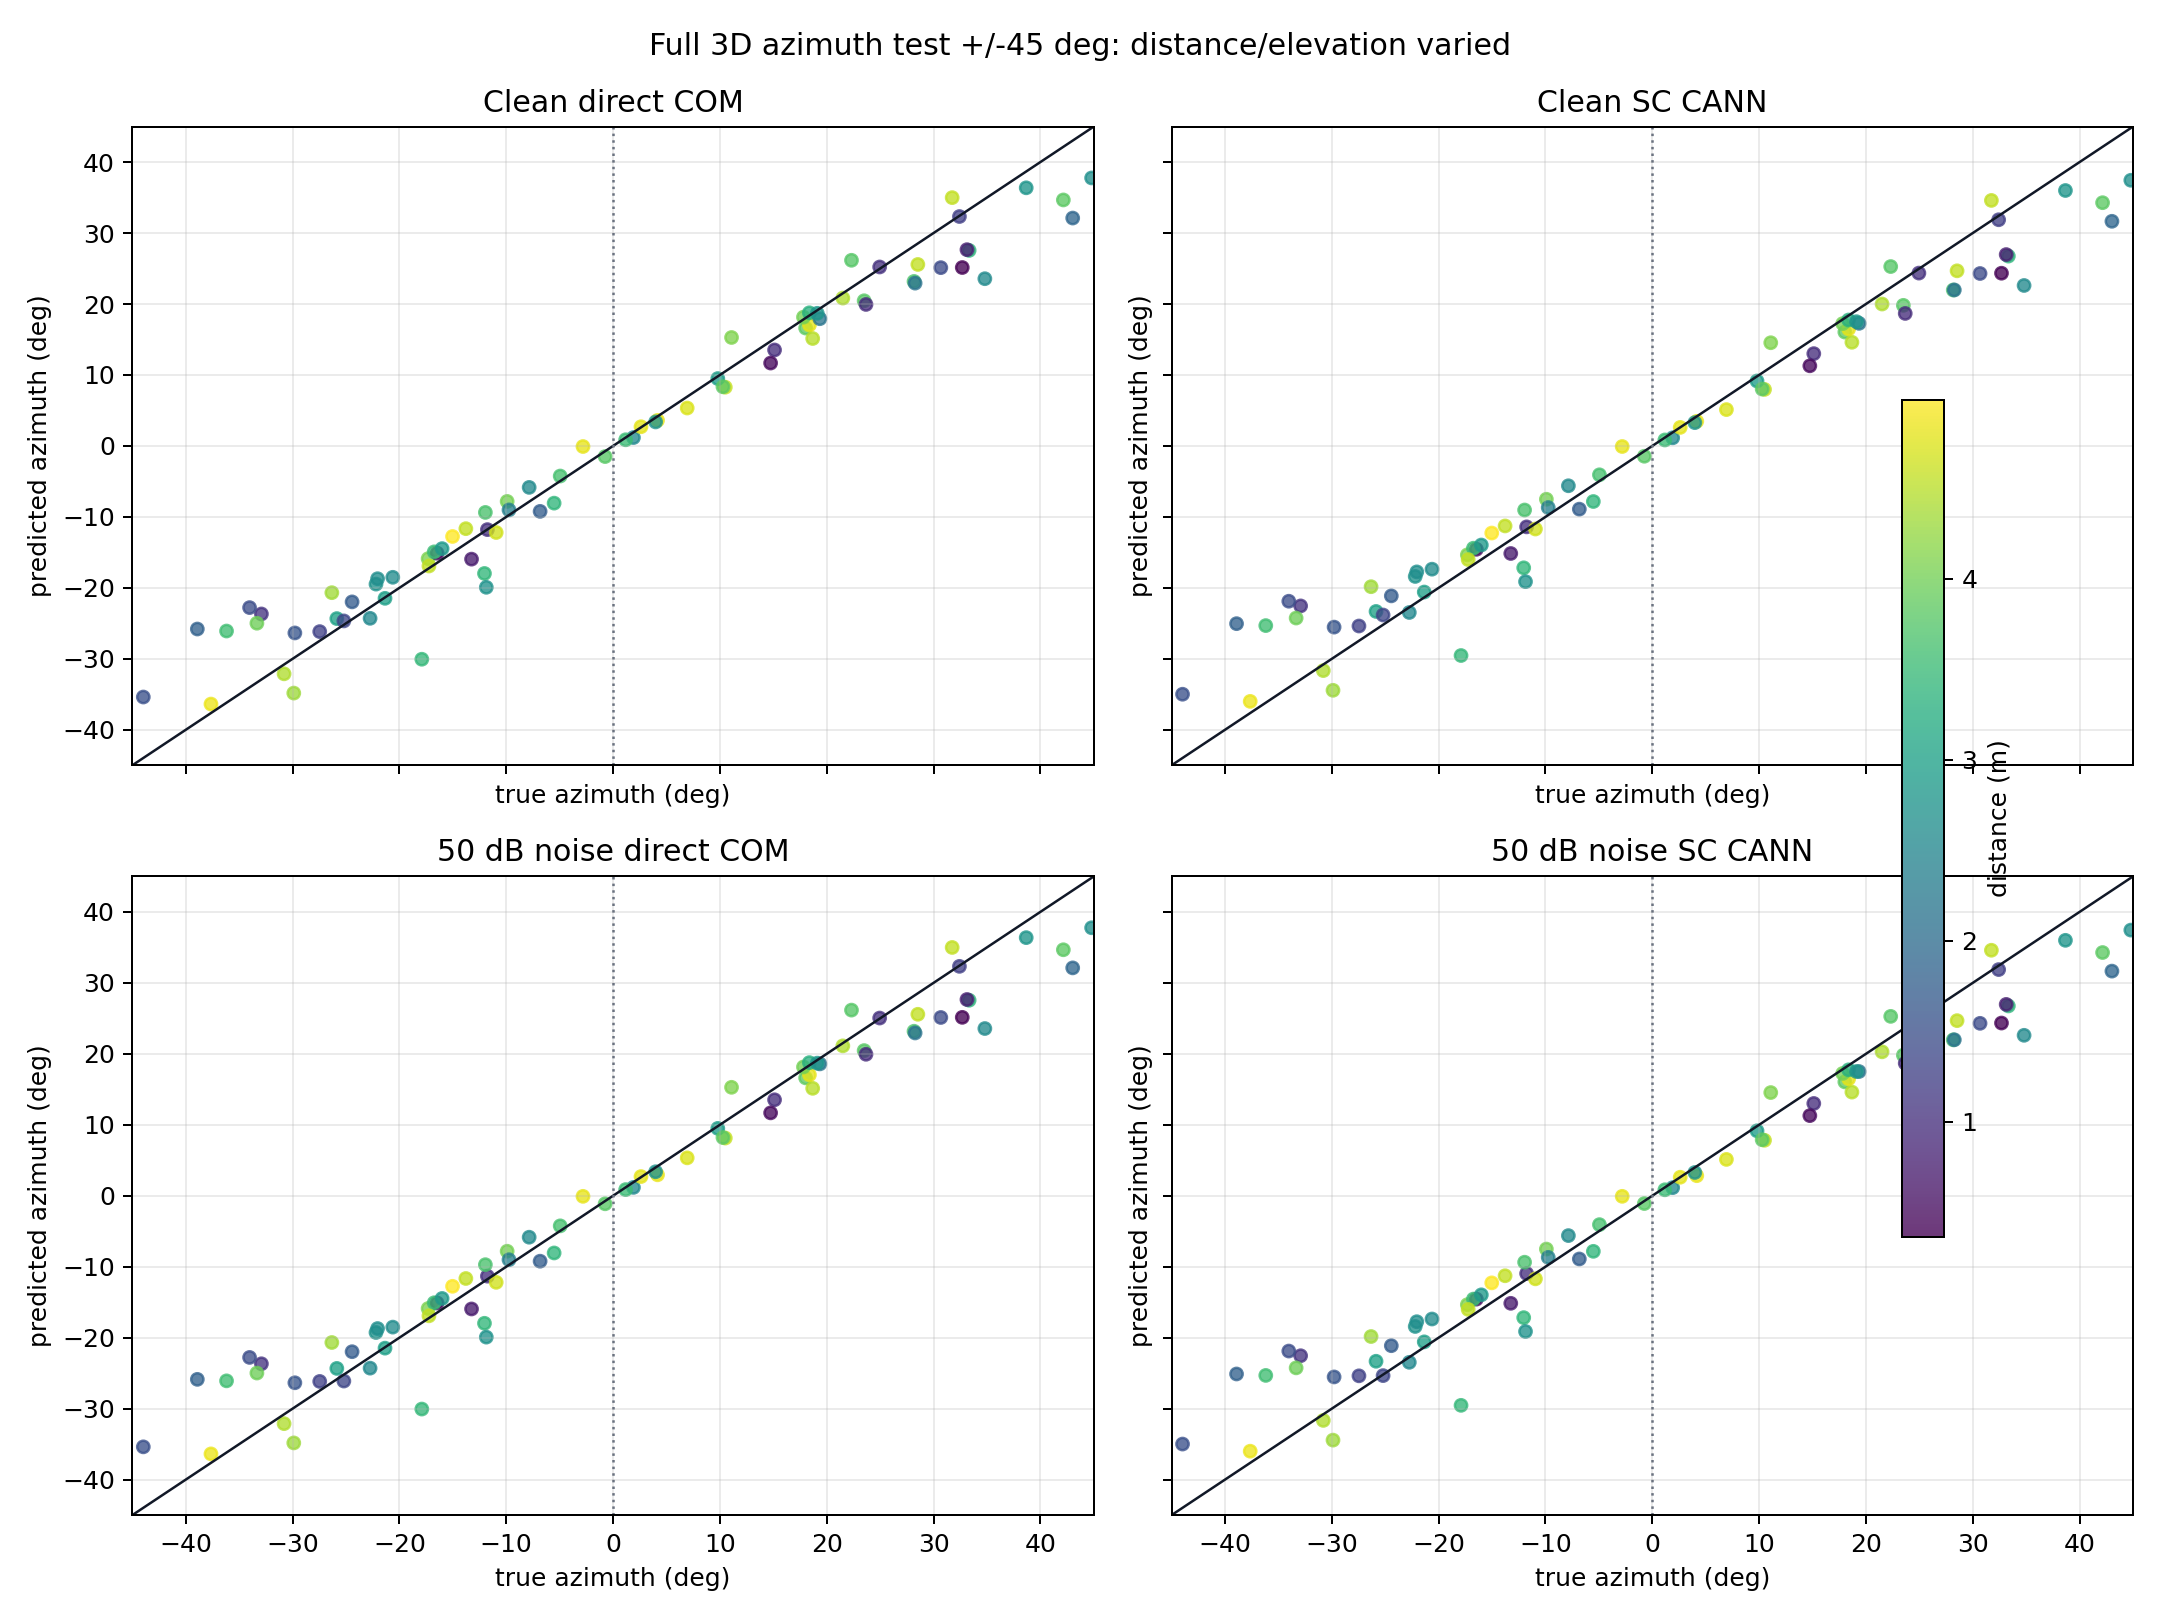
\includegraphics[width=1\textwidth]{4_Results/azimuth/ITD_scatter.png}
    \caption{Scatters showing results of ITD based azimuth estimation for constrained 3D environment, with direct and CANN readouts, in clean and noisy environments}
    \label{fig:ITD_scatter}
\end{figure}




\section{Elevation Pathway}

The elevation pathway went through the largest design progression. Early tests used a local-dip disinhibition model, where each candidate elevation was associated with an expected notch frequency and the readout looked for local spectral suppression. This captured the intuition of notch detection but used too little of the transfer-function structure. Later models compared the full observed spectral profile against candidate comb-filter templates, and then added signal-weighted synaptic weights so that notches in high-energy frequency regions contributed more than notches in weak parts of the emitted sweep.

\begin{table}[H]
    \centering
    \caption{Elevation pathway design progression. Only the centre-of-mass readouts are shown to keep the comparison focused.}
    \label{tab:elevation_design_progression}
    \small
    \begin{tabular}{lrrrr}
        \toprule
        Readout & MAE & RMSE & Max error & Bias \\
        \midrule
        Local-dip disinhibition COM & 16.907$^\circ$ & 21.114$^\circ$ & 52.718$^\circ$ & -9.858$^\circ$ \\
        Explicit E/I weight-profile COM & 7.099$^\circ$ & 8.828$^\circ$ & 18.090$^\circ$ & 2.299$^\circ$ \\
        Baseline-equalised full-transfer DCN COM & 5.181$^\circ$ & 6.182$^\circ$ & 10.830$^\circ$ & 2.913$^\circ$ \\
        Signal-weighted full-transfer DCN COM & 3.137$^\circ$ & 3.777$^\circ$ & 7.244$^\circ$ & 1.070$^\circ$ \\
        Deep-comb baseline-equalised DCN COM & 4.837$^\circ$ & 5.724$^\circ$ & 9.879$^\circ$ & 2.611$^\circ$ \\
        Deep-comb signal-weighted DCN COM & 2.824$^\circ$ & 3.377$^\circ$ & 6.491$^\circ$ & 0.814$^\circ$ \\
        First-notch diagnostic readout & 2.894$^\circ$ & 3.981$^\circ$ & 12.257$^\circ$ & -2.764$^\circ$ \\
        \bottomrule
    \end{tabular}
\end{table}

The progression in Table~\ref{tab:elevation_design_progression} shows why the final DCN-style model uses the full transfer template rather than a single notch detector. The first-notch diagnostic performs well in MAE, but it is an engineered control rather than a neural population model: it explicitly reads off a notch location. The deep-comb signal-weighted DCN achieves slightly lower MAE and substantially lower maximum error while still being expressible as a population of template-sensitive neurons.

The signal weighting is important even though the observed spectrum is normalised by the baseline no-notch spectrum. Baseline equalisation estimates the relative transfer shape, but it does not make all frequencies equally reliable. A normalised dip in a low-energy part of the chirp is still less trustworthy than a dip in a high-energy part of the call. Weighting the mismatch by the baseline signal envelope and expected notch depth therefore improves both accuracy and bias.

The CANN alone makes only a small difference to the elevation pathway. The major improvement comes from applying inverse-sigmoid calibration after the population readout. This implies that the DCN population contains the correct ordering information, but the scalar readout is systematically warped. The best elevation result is obtained when the reflected CANN readout is combined with this calibration, reducing the full-3D MAE to 0.938$^\circ$.


\begin{figure}[H]
    \centering
    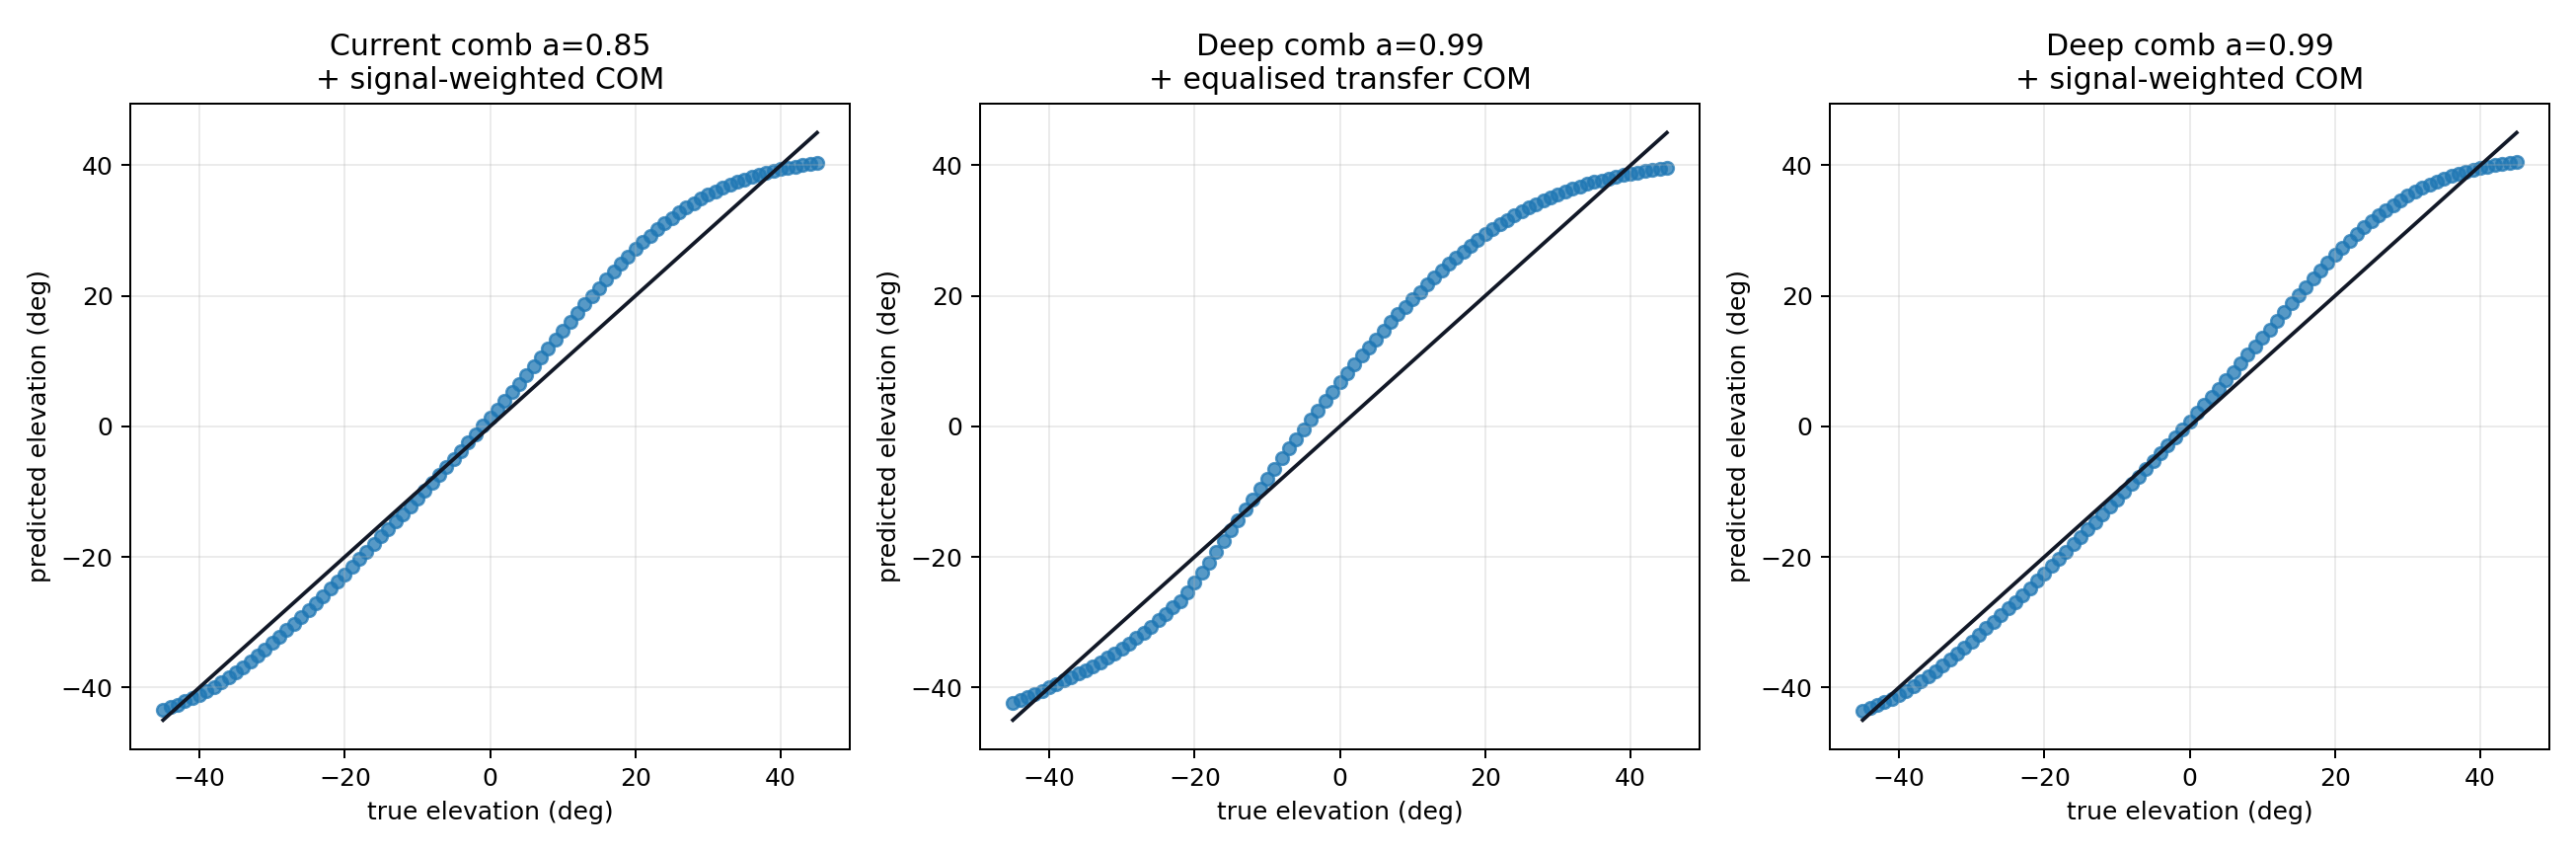
\includegraphics[width=1\textwidth]{4_Results/elevation/deep_comb.png}
    \caption{Elevation scatter plots for elevation showing effect of signal weighting and deep comb}
    \label{fig:deep_comb}
\end{figure}


\begin{figure}[H]
    \centering
    
\includegraphics[width=1\textwidth]{4_Results/elevation/warp_scatter.png}
    \caption{Elevation scatter plots for elevation showing effect of warping}
    \label{fig:el_warp_scatter}
\end{figure}

\section{CANN summary results}

\begin{figure}[H]
    \centering
    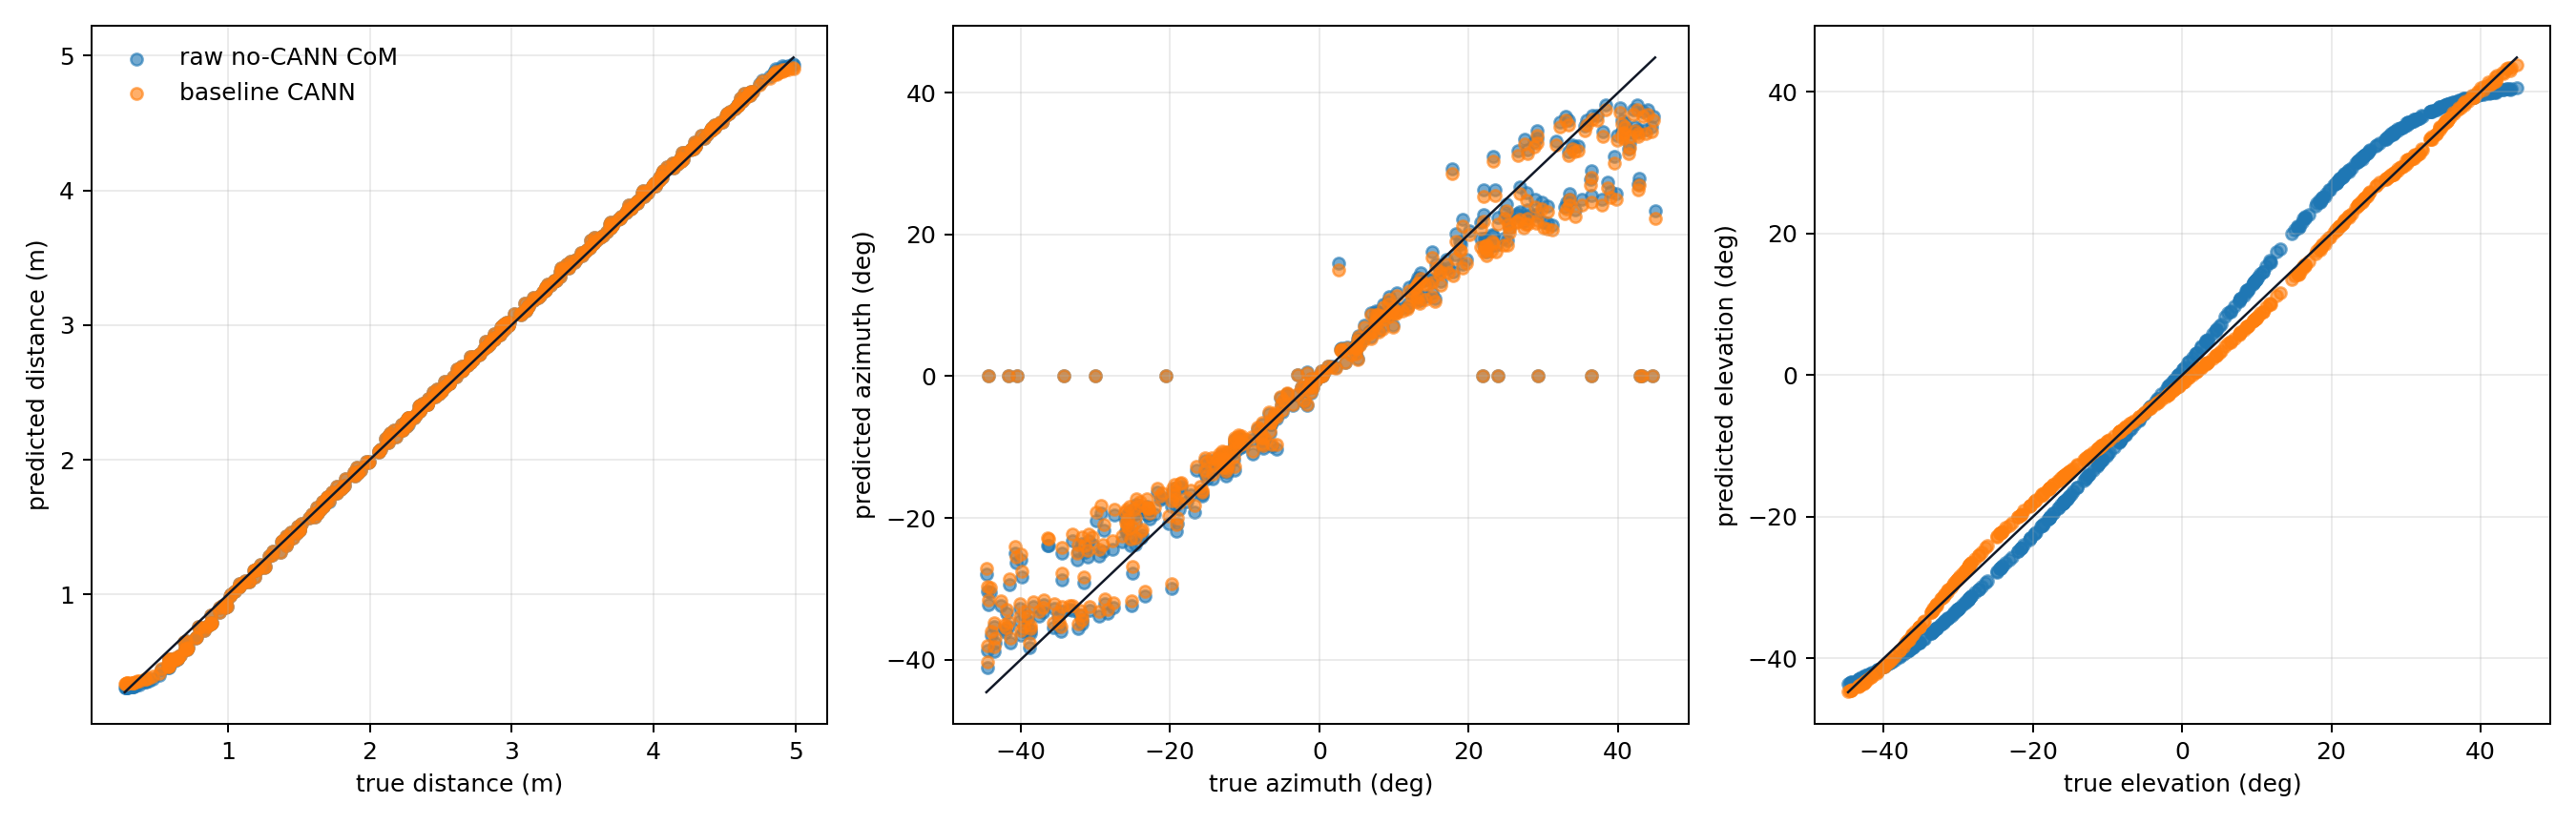
\includegraphics[width=1\textwidth]{4_Results/CANN_final/clean.png}
    \caption{Scatter plots comparing CANN vs direct `raw' readout estimates for noise-free signals}
    \label{fig:CANN_scatter_clean}
\end{figure}

\begin{figure}[H]
    \centering
    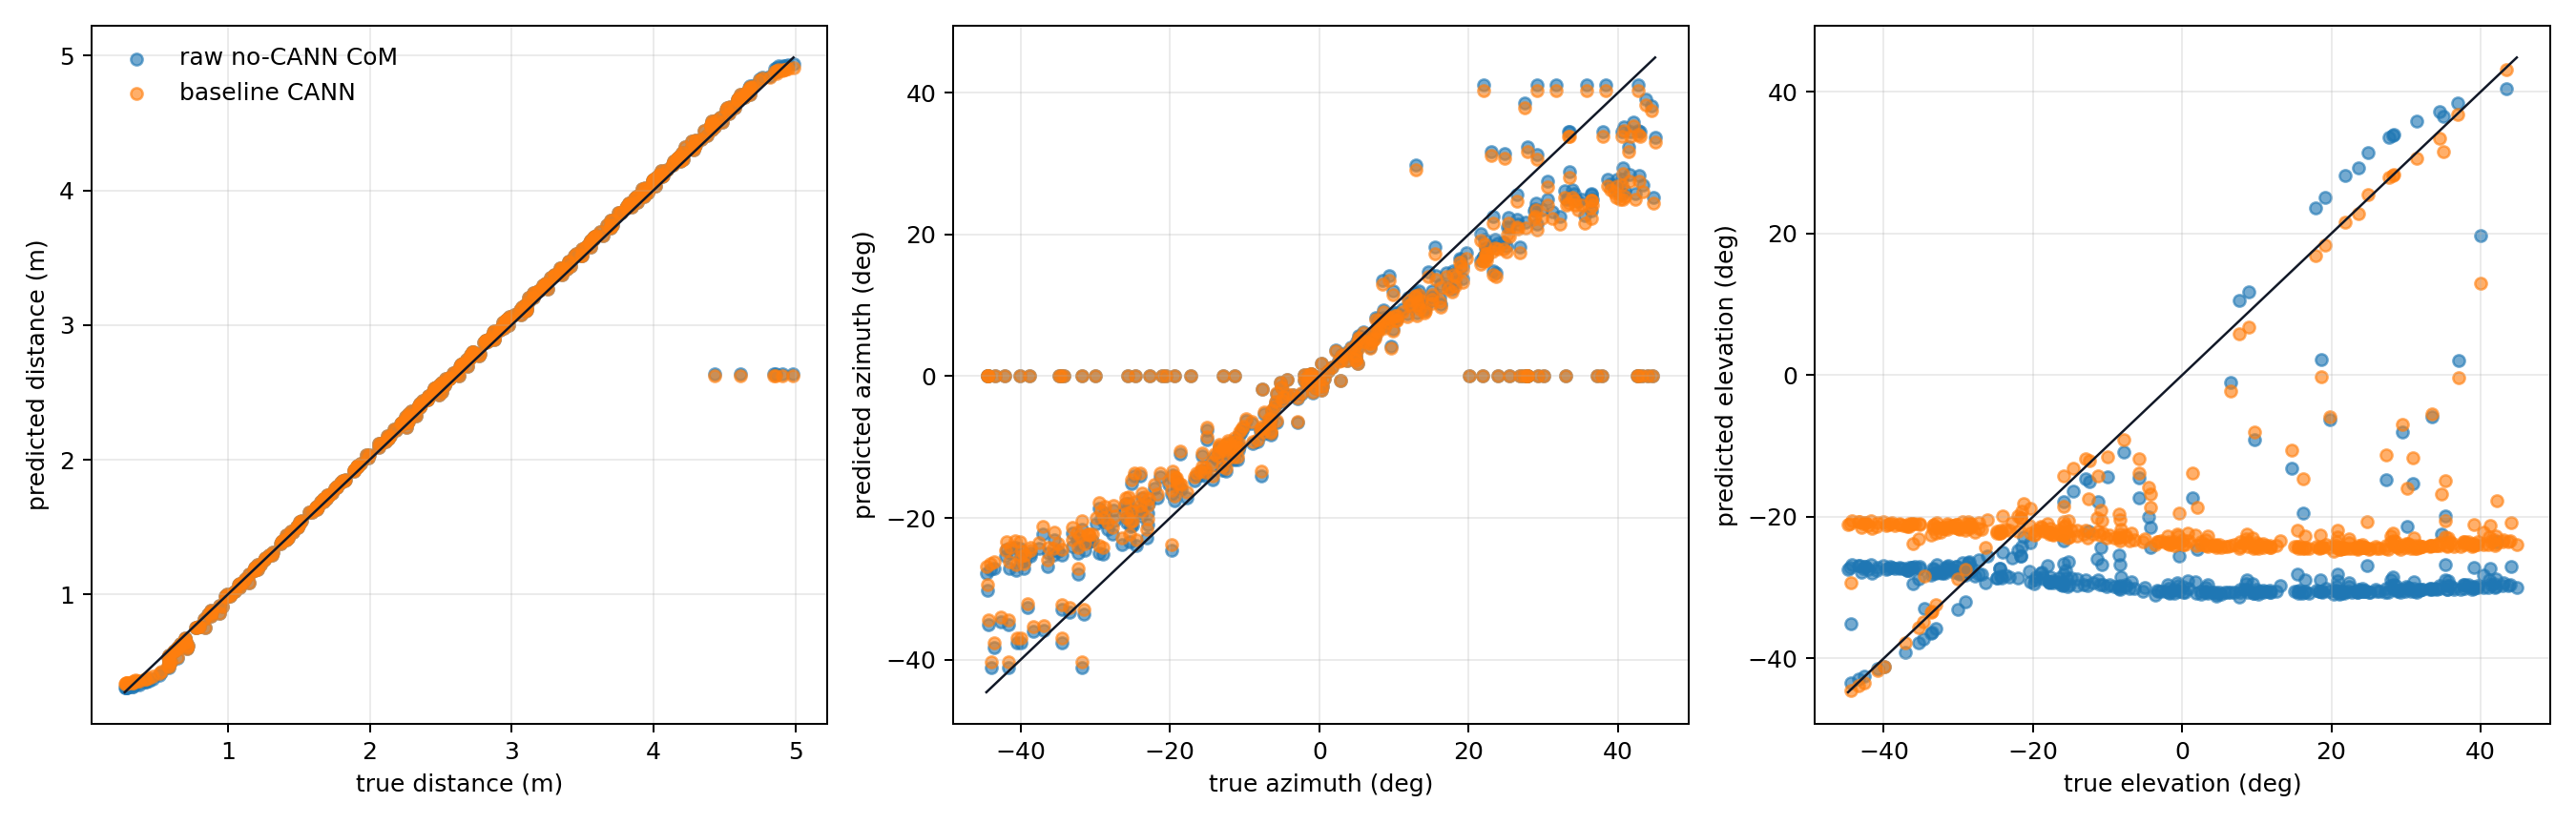
\includegraphics[width=1\textwidth]{4_Results/CANN_final/noise.png}
    \caption{Scatter plots comparing CANN vs direct `raw' readout estimates for noisy signals}
    \label{fig:CANN_scatter_noise}
\end{figure}

\begin{figure}[H]
    \centering
    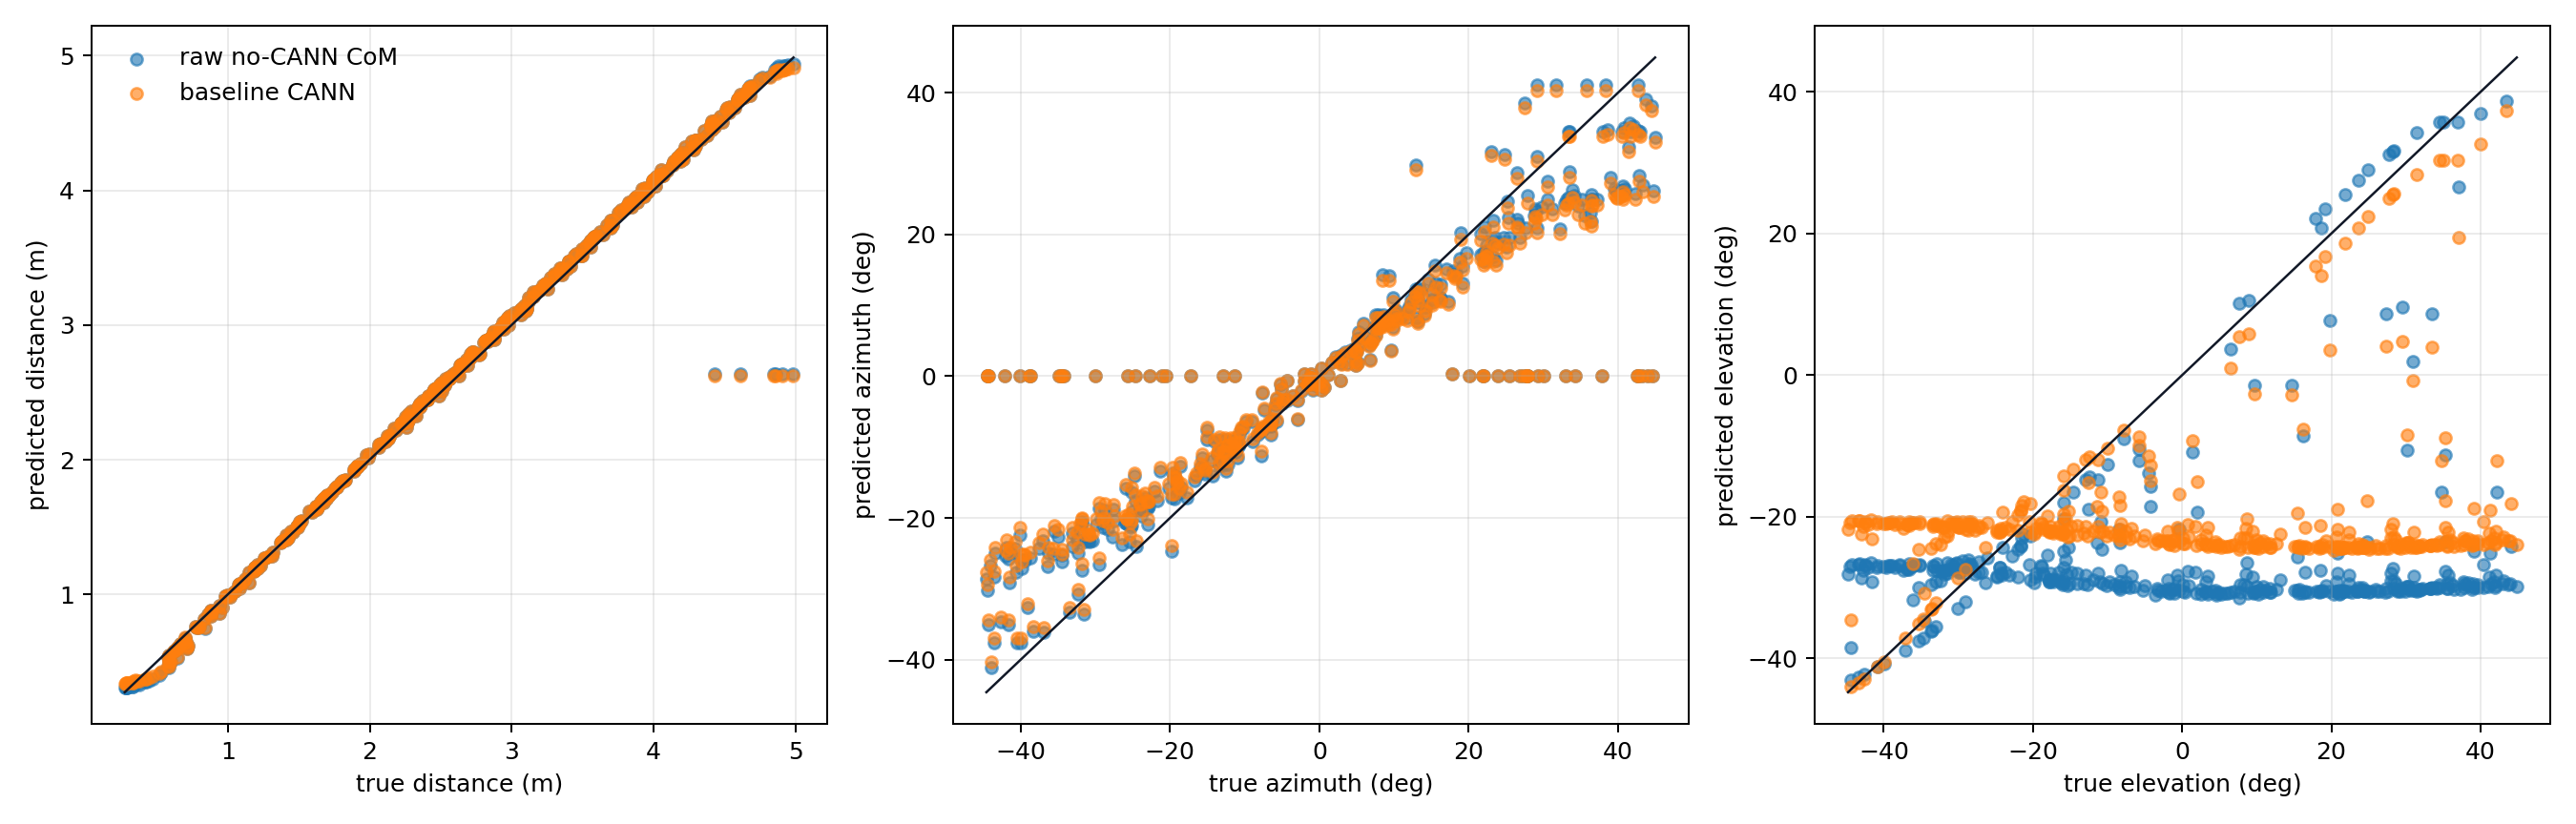
\includegraphics[width=1\textwidth]{4_Results/CANN_final/reverb.png}
    \caption{Scatter plots comparing CANN vs direct `raw' readout estimates for noisy signals with multiple delayed echoes}
    \label{fig:CANN_scatter_reverb}
\end{figure}




\section{Trainable SNN Baselines}

The trainable fusion model must be compared against simpler trained SNN baselines. Otherwise, improved performance could simply be due to the use of any trainable network, rather than the structured auditory pathways. Two input-only baselines were therefore tested. The raw-waveform baseline receives the binaural acoustic waveform directly. The cochlear-raster baseline receives the binaural spike raster produced by the cochlear front end. Each was tested in a projected version, where the high-dimensional input is compressed before entering the SNN, and a direct version, where the flattened input is passed directly to the same style of readout network.

\begin{table}[H]
    \centering
    \caption{Input-only SNN baselines. These models use the same output representation and loss structure as the final trainable readout, but do not receive the hand-designed pathway populations.}
    \label{tab:snn_input_baselines}
    \resizebox{\linewidth}{!}{%
    \begin{tabular}{llrrrrrr}
        \toprule
        Condition & Baseline & Input dim. & Parameters & Distance MAE & Azimuth MAE & Elevation MAE & Combined error \\
        \midrule
        Clean & Raw waveform, projected & 474 & 55,597 & 0.2954~m & 21.160$^\circ$ & 20.221$^\circ$ & 0.3262 \\
        Clean & Raw waveform, direct & 4608 & 452,461 & 0.8053~m & 21.580$^\circ$ & 22.855$^\circ$ & 0.3828 \\
        Clean & Cochlear raster, projected & 474 & 55,597 & 0.0677~m & 4.292$^\circ$ & 6.282$^\circ$ & 0.0828 \\
        Clean & Cochlear raster, direct & 960 & 102,253 & 0.0651~m & 6.033$^\circ$ & 7.178$^\circ$ & 0.1022 \\
        \midrule
        Environmental noise & Raw waveform, projected & 474 & 55,597 & 0.4113~m & 23.106$^\circ$ & 22.667$^\circ$ & 0.3665 \\
        Environmental noise & Raw waveform, direct & 4608 & 452,461 & 0.9794~m & 23.847$^\circ$ & 23.836$^\circ$ & 0.4185 \\
        Environmental noise & Cochlear raster, projected & 474 & 55,597 & 0.0733~m & 6.235$^\circ$ & 4.987$^\circ$ & 0.0880 \\
        Environmental noise & Cochlear raster, direct & 960 & 102,253 & 0.0699~m & 5.991$^\circ$ & 4.678$^\circ$ & 0.0837 \\
        \midrule
        Noise + reverb & Raw waveform, projected & 474 & 55,597 & 0.3945~m & 22.349$^\circ$ & 22.307$^\circ$ & 0.3571 \\
        Noise + reverb & Raw waveform, direct & 4608 & 452,461 & 0.9414~m & 21.990$^\circ$ & 22.471$^\circ$ & 0.3921 \\
        Noise + reverb & Cochlear raster, projected & 474 & 55,597 & 0.0772~m & 5.415$^\circ$ & 3.811$^\circ$ & 0.0735 \\
        Noise + reverb & Cochlear raster, direct & 960 & 102,253 & 0.0632~m & 5.900$^\circ$ & 4.704$^\circ$ & 0.0828 \\
        \bottomrule
    \end{tabular}%
    }
\end{table}

The raw-waveform SNN baselines perform poorly, even when given many more parameters. This suggests that the training set is not large enough for a small SNN to learn the full signal-processing stack directly from waveform samples. The cochlear-raster baselines are much stronger, showing that the cochlear front end is a useful representation even without the later biological pathways. However, they still underperform the final structured readout in the full comparison below. This supports the main modelling claim: the hand-designed auditory pathways are not merely decorative biological detail, but provide useful intermediate features for the final trainable network.



\section{Full Model Comparison}

The final comparison uses the constrained operating region of 0.25--5~m and $\pm45^\circ$ azimuth/elevation. Three environmental conditions are shown. The clean case has no environmental noise. The environmental-noise case adds a 50~dB acoustic noise field before the binaural HRTF and elevation filtering stages, making it a harsher and more physically fair test than adding receiver noise after the cue generation. The noise-plus-reverb case adds the same environmental noise together with delayed echo/reverberation components.

Four structured readouts are compared. The raw readout uses direct centre-of-mass decoding from the pathway populations, before CANN correction. The fixed baseline uses the CANN and calibration readouts without trainable fusion. The direct SNN readout predicts the full coordinate vector directly from the cached pathway features. The residual SNN readout predicts a correction to the fixed pathway estimate.

\begin{table}[H]
    \centering
    \caption{Full-model comparison in the constrained 0.25--5~m, $\pm45^\circ$ test region. The best input-only SNN baseline is included for each condition to compare the structured model against a trainable SNN without handcrafted pathway features.}
    \label{tab:full_model_results}
    \resizebox{\linewidth}{!}{%
    \begin{tabular}{llrrrrr}
        \toprule
        Condition & Readout & Distance MAE & Azimuth MAE & Elevation MAE & Euclidean MAE & Combined error \\
        \midrule
        Clean & Best input-only SNN & 0.0677~m & 4.292$^\circ$ & 6.282$^\circ$ & 0.2580~m & 0.0828 \\
        Clean & Raw pathway COM & 0.0365~m & 4.580$^\circ$ & 2.986$^\circ$ & 0.2999~m & 0.0585 \\
        Clean & Fixed CANN baseline & 0.0366~m & 4.925$^\circ$ & 0.910$^\circ$ & 0.2435~m & 0.0457 \\
        Clean & Direct SNN on pathway features & 0.0624~m & 2.449$^\circ$ & 1.133$^\circ$ & 0.1612~m & 0.0307 \\
        Clean & Residual SNN on pathway features & 0.0139~m & 2.619$^\circ$ & 0.267$^\circ$ & 0.1247~m & 0.0223 \\
        \midrule
        Environmental noise & Best input-only SNN & 0.0699~m & 5.991$^\circ$ & 4.678$^\circ$ & 0.2830~m & 0.0837 \\
        Environmental noise & Raw pathway COM & 0.0786~m & 7.691$^\circ$ & 29.980$^\circ$ & 1.7054~m & 0.2843 \\
        Environmental noise & Fixed CANN baseline & 0.0789~m & 8.094$^\circ$ & 26.642$^\circ$ & 1.5772~m & 0.2626 \\
        Environmental noise & Direct SNN on pathway features & 0.0690~m & 3.831$^\circ$ & 4.018$^\circ$ & 0.3214~m & 0.0627 \\
        Environmental noise & Residual SNN on pathway features & 0.0213~m & 3.705$^\circ$ & 3.505$^\circ$ & 0.2968~m & 0.0548 \\
        \midrule
        Noise + reverb & Best input-only SNN & 0.0772~m & 5.415$^\circ$ & 3.811$^\circ$ & 0.3001~m & 0.0735 \\
        Noise + reverb & Raw pathway COM & 0.0796~m & 7.736$^\circ$ & 28.962$^\circ$ & 1.6917~m & 0.2771 \\
        Noise + reverb & Fixed CANN baseline & 0.0799~m & 8.147$^\circ$ & 25.975$^\circ$ & 1.5674~m & 0.2581 \\
        Noise + reverb & Direct SNN on pathway features & 0.0731~m & 3.883$^\circ$ & 4.028$^\circ$ & 0.3431~m & 0.0635 \\
        Noise + reverb & Residual SNN on pathway features & 0.0202~m & 3.898$^\circ$ & 3.341$^\circ$ & 0.3103~m & 0.0550 \\
        \bottomrule
    \end{tabular}%
    }
\end{table}

The clean-condition results show that the fixed pathway model is already functional. Raw pathway decoding gives 3.65~cm distance MAE, 4.580$^\circ$ azimuth MAE, and 2.986$^\circ$ elevation MAE. Adding the fixed CANN/calibrated baseline improves the elevation error to 0.910$^\circ$ and reduces Euclidean error from 0.2999~m to 0.2435~m. This is consistent with the pathway-level results: the CANN/calibration stage is most useful for elevation, while distance and azimuth are mainly determined upstream.

The environmental-noise results reveal the main weakness of the fixed model. The raw and fixed baseline readouts suffer a large elevation collapse, with elevation MAE rising to 29.980$^\circ$ and 26.642$^\circ$ respectively. This occurs because environmental noise is added before the binaural and elevation cue transformations, so it is shaped by the same HRTF and comb-filter stages as the signal. The noise therefore corrupts the spectral cue itself rather than simply adding independent receiver noise after the cue has been formed.

The trainable SNN fusion readouts substantially reduce this failure. Under environmental noise, the residual SNN reduces combined error from 0.2626 for the fixed baseline to 0.0548, and reduces Euclidean MAE from 1.5772~m to 0.2968~m. The direct SNN readout is also strong, but the residual version gives the best combined error in all three conditions. This supports the residual formulation: the hand-designed pathways provide a good coordinate estimate, and the SNN learns systematic corrections when the cues interact or fail.

The noise-plus-reverb result is also informative. Adding delayed echo/reverberation components does not destroy the residual model: combined error remains almost unchanged, increasing only from 0.0548 to 0.0550. This suggests that, in the constrained region, the final trainable readout is more limited by spectral cue corruption from environmental noise than by the added late echoes used in this test.

The best input-only SNN baselines are competitive with the fixed CANN baseline under noisy conditions, but they remain worse than the residual pathway-feature SNN. This is the key comparison for the project aim. A small SNN can learn useful localisation behaviour from cochlear spike rasters, but it performs better when it receives structured distance, azimuth, elevation, CANN, and confidence features from the biologically motivated pathways. The final model therefore benefits from both parts of the design: explicit auditory feature extraction and limited trainable contextual integration.

\begin{figure}[H]
    \centering
    
\includegraphics[width=1\textwidth]{4_Results/trained/clean.png}
    \caption{Scatter plots comparing a CANN baseline, residually trained, and directly trained model estimates for noise-free signals}
    \label{fig:trained_scatter_clean}
\end{figure}

\begin{figure}[H]
    \centering
    
\includegraphics[width=1\textwidth]{4_Results/trained/noise.png}
    \caption{Scatter plots comparing a CANN baseline, residually trained, and directly trained model estimates for noisy signals}
    \label{fig:trained_scatter_noise}
\end{figure}

\begin{figure}[H]
    \centering
    
\includegraphics[width=1\textwidth]{4_Results/trained/reverb.png}
    \caption{Scatter plots comparing a CANN baseline, residually trained, and directly trained model estimates for noisy signals with multiple delayed echoes}
    \label{fig:trained_scatter_reverb}
\end{figure}

\begin{figure}[H]
    \centering
    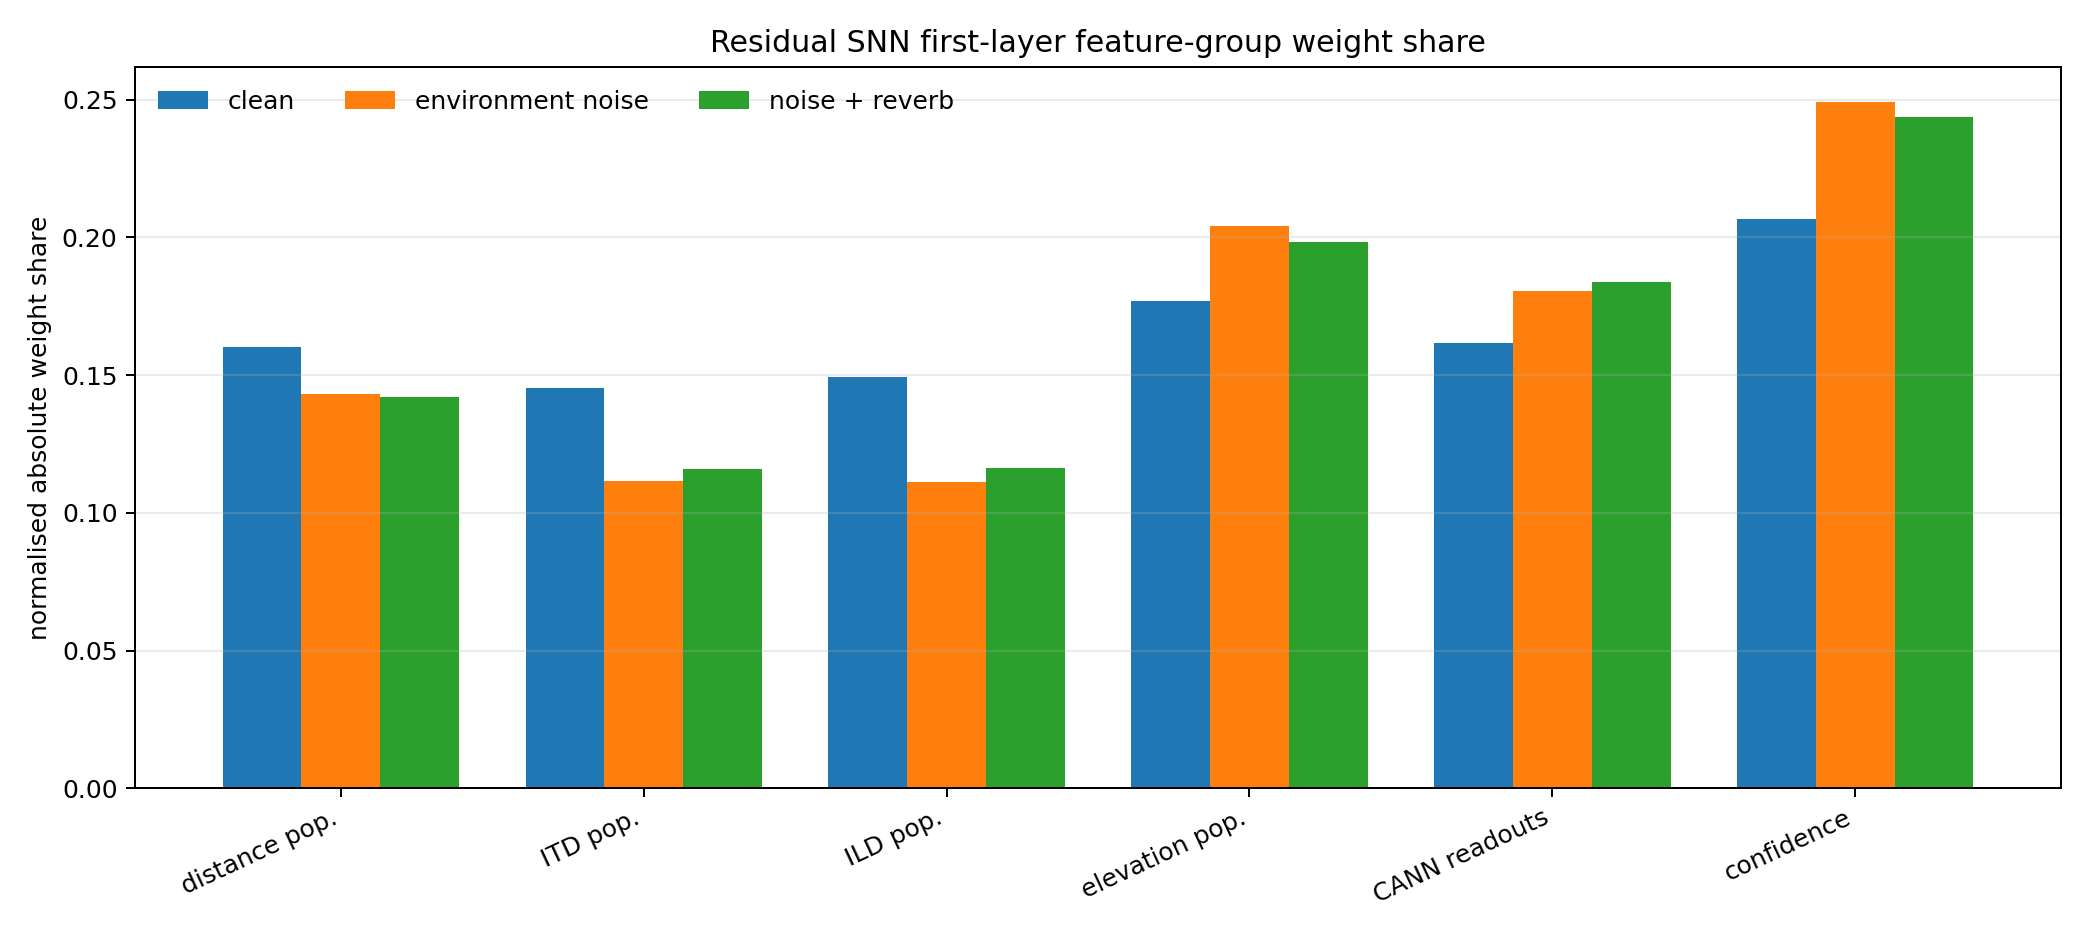
\includegraphics[width=1\textwidth]{4_Results/trained/residual_weights.png}
    \caption{First layer weights of the residual SNN as a proxy for importance}
    \label{fig:trained_scatter_noise}
\end{figure}

\begin{figure}[H]
    \centering
    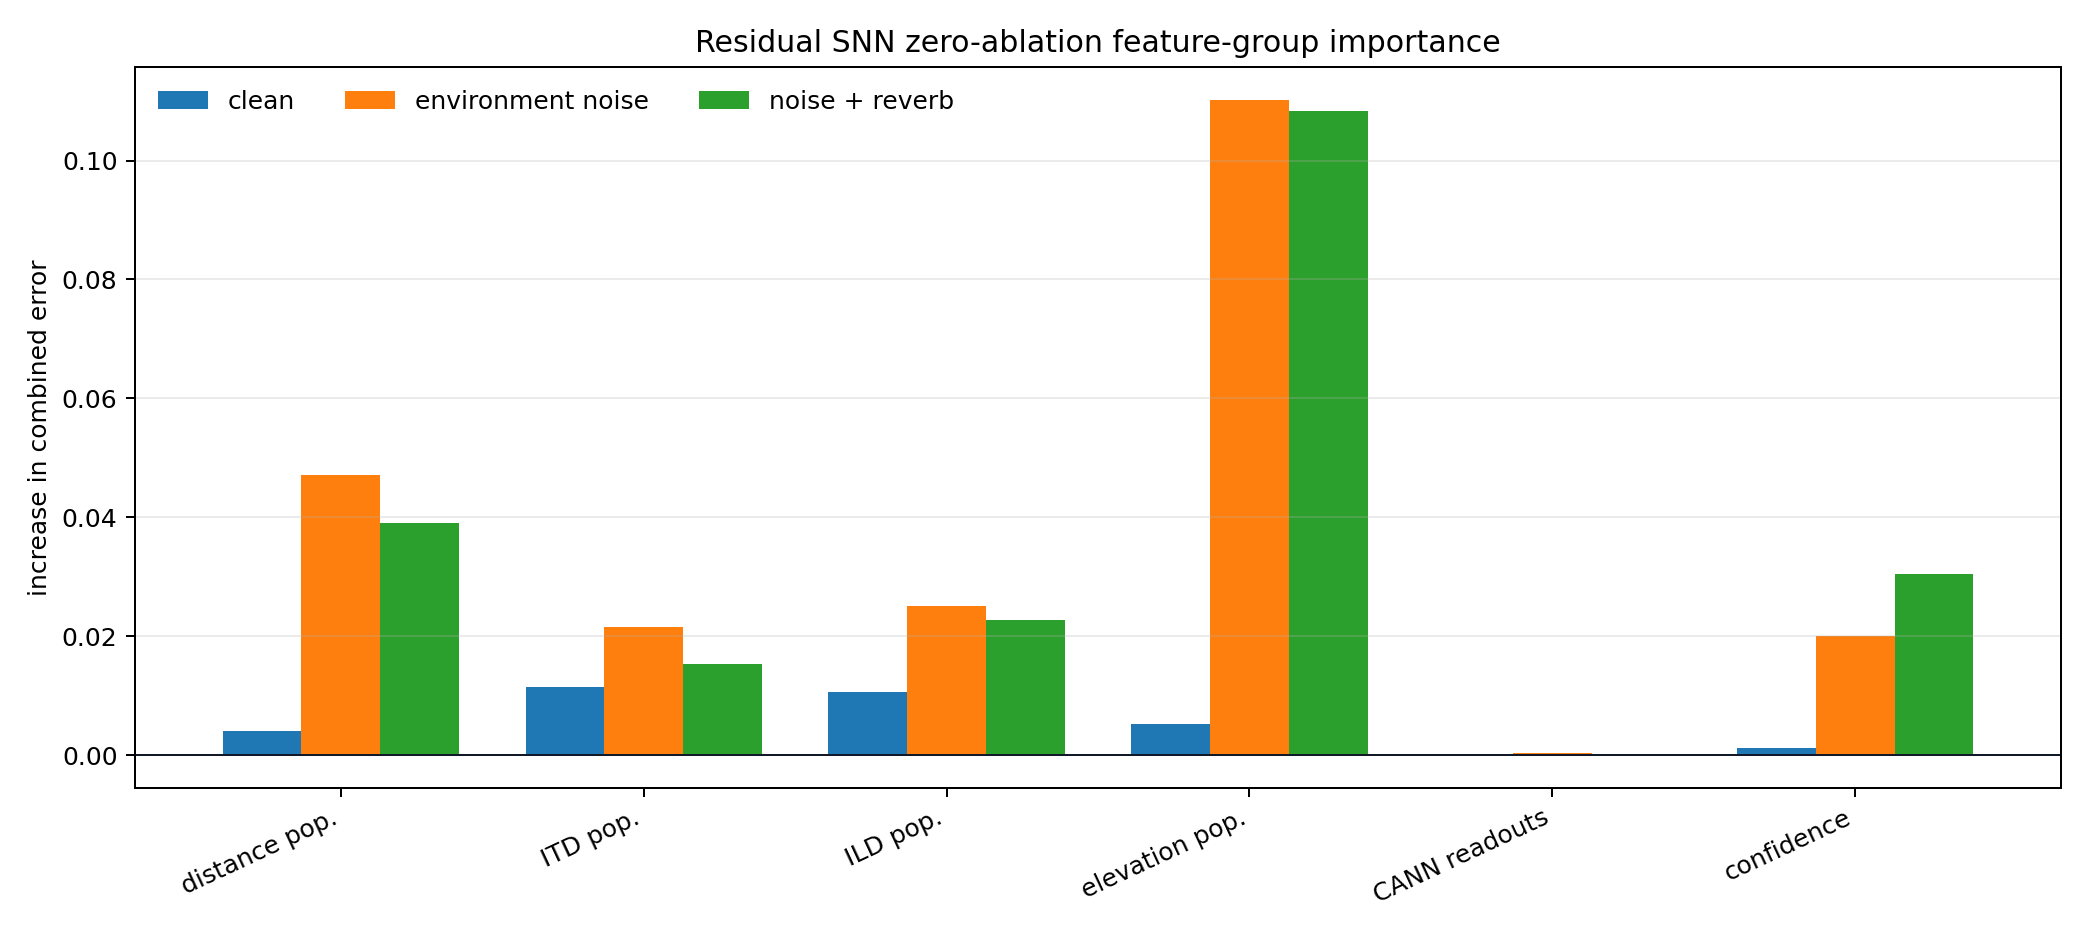
\includegraphics[width=1\textwidth]{4_Results/trained/residual_ablation.png}
    \caption{Test data ablation study as a proxy for importance}
    \label{fig:trained_scatter_reverb}
\end{figure}



\section{Discussion}

The results support three conclusions. First, the individual pathways solve different parts of the localisation problem with different reliability. Distance is the most stable in the constrained region because time-of-flight is a strong cue and the pathway is directly tuned to the 0.25--5~m range. Azimuth is cue-dependent: ILD is accurate when isolated and calibrated, but ITD is more robust in the full 3D setting. Elevation is the most sensitive to modelling choices because it depends on spectral shape rather than a simple delay or binaural imbalance.

Second, the CANN is useful but not sufficient on its own. It acts as a population stabiliser and readout mechanism, not as a general error-correction algorithm. It improves distance slightly, improves elevation when paired with calibration, and can slightly worsen azimuth if the input population is already sharp. This is why the final trainable model keeps both raw populations and CANN readouts rather than forcing all information through the attractor scalar.

Third, the final residual SNN is best interpreted as contextual integration. It does not learn echolocation from scratch. Instead, it receives interpretable pathway populations and learns how to combine them when cues interact. This is biologically and engineering-wise preferable to a pure black-box readout: the lower pathways remain inspectable, while the final stage handles systematic cross-cue errors that are difficult to remove manually.

There are also clear limitations. The strongest reported results are in the constrained operating region for which the model was tuned. Expanded-range distance testing shows that the model degrades outside this region. The environmental-noise tests also show that the fixed elevation pathway remains vulnerable when the spectral cue is corrupted before HRTF and comb filtering. Finally, the trainable SNN results depend on cached simulated data rather than measured acoustic recordings, so the next step would be to test whether the same pathway structure transfers to more realistic HRTFs, target reflections, and cluttered multi-object scenes.



\writingbox{TO DO

Literature benchmarks

General literature review: \cite{Danneville2024ASystems}
Quote: The question of distance estimation is not studied in any works apart from [DOA: \cite{Dalmas2024NeuromorphicEstimation}], which reported incorrect distances from ITD only, and the study by Roozbehi et al. [Reservoir: \cite{RoozbehiDateLocalization}], which gave spatial coordinates but constrained to within the baseline of the microphone array.
Otherwise gives varying results which are hard to compare given the very different setups.

DOA: \cite{Dalmas2024NeuromorphicEstimation}, got 1 degrees resolution with ACC 71.3\% using natural sounds and quiet test environment (simulation), according to \cite{Dalmas2024NeuromorphicEstimation}

Reservoir: \cite{RoozbehiDateLocalization}, got 69.8\% ACC 3.4◦MAE 0.38 m MAE (2D) in a noist test environment (simulation), according to \cite{Dalmas2024NeuromorphicEstimation}

Matsuo: \cite{Matsuo2013EcholocationSound}
Resistive memories: \cite{Moro2022NeuromorphicTransducers}

Benchmark Class & Reference,Environment Type,Architecture Type,Key Metric / Error Floor,Strategic Thesis Application
"DOA Target[Dalmas et al., 2024](IEEE Trans. Instrum. Meas.)",Simulated(Python model evaluated using real indoor acoustic recordings),Spike-Based Algorithm(Non-ML; Hassenstein-Reichardt spike coincidence model),84\% localization accuracy within an error margin of ±5° (1–3 m range),Benchmarks your Azimuth & Elevation MAE; demonstrates that biological coincidence line frameworks achieve sub-degree angular capabilities.
"Sterile Ranging Baseline[Matsuo, 2013](Frontiers in Physiology)",Simulated(Fully digital acoustic environment),Classical DSP(Non-spiking; mathematical cross-correlation model of FM sweeps),Exceptional sub-millimeter ranging precision (~0.22 mm or 1.3 µs delay error),Highlights why your project prioritizes noise-robustness over sterile geometric precision; rigid cross-correlation pipelines collapse outside of pristine environments.
"Dynamic Sound Localization[Roozbehi et al., 2024](IEEE Access)",Simulated(Python model evaluated using real-world multi-microphone environmental audio),Trainable SNN(Reservoir SNN utilizing dynamic size adjustment and plastic node re-allocation),Noise-robust tracking; successfully resolves complex front-back spatial ambiguities,Proves that your Fixed-Path + Residual layout is structurally lighter; you achieve noise robustness without the heavy computational overhead of dynamic node re-allocation.
"Neuromorphic Edge Baseline[Nature Comm, 2022]",Physical Hardware(Custom silicon chip coupled to physical ultrasonic transducers),Hardware SNN(Memristive resistive crossbar circuit executing barn-owl computational maps),"Centimeter-level spatial tracking; explicitly fragile to device non-idealities, hardware drift, and noise",Justifies your Trainable Residual Layer; proves that physical neuromorphic hardware requires a software error-corrector to survive real-world deployment conditions.
Your Model(Proposed BI-SNN Framework),Simulated(Complete modular software-based echolocation environment),Hybrid Architecture(Fixed biomimetic SNN pathways coupled to a trainable residual SNN stage),1.4 cm absolute distance MAE in clean settings; stays highly stable at 2.1 cm in 50 dB SNR noise,The Core Contribution: Demonstrates high data efficiency and structural interpretability while entirely eliminating the noise-vulnerability of pure biological networks.


Biological baselines:
It has been shown that FM-bats can discriminate differences in echo delay, the cue for target distance, of less than 60 microseconds \cite{Simmons1973TheBats}. This gives us a biological baseline for distance

Tho others have shown lower:
0.3mm \cite{Kanwal2007AuditoryCommunication}
less than 0.1mm \cite{Ulanovsky2009IntroductionSemester}
1-2 degrees for azimuth \cite{Ulanovsky2009IntroductionSemester}
3 degrees for elevation \cite{Lawrence1982EcholocationTargets}


}